\documentclass[11pt]{amsart}
%\documentclass[11pt]{article}
\usepackage{geometry}                % See geometry.pdf to learn the layout options. There are lots.
\geometry{letterpaper, width=7in, height=9in}                   % ... or a4paper or a5paper or ... 
\usepackage{graphicx}
\usepackage{pdfpages}
\usepackage{amssymb}
\usepackage{epstopdf}
\usepackage{color}
\usepackage{hyperref}
\usepackage{courier}
\usepackage{listings}

\usepackage{siunitx}
\usepackage{booktabs}

\let\oldsection\section
\renewcommand\section{\clearpage\oldsection}

\DeclareGraphicsRule{.tif}{png}{.png}{`convert #1 `dirname #1`/`basename #1 .tif`.png}
\DeclareGraphicsRule{.gif}{pdf}{.pdf}{`convert #1 `dirname #1`/`basename #1 .gif`.pdf}

   \newsavebox{\fmbox}
   \newenvironment{fmpage}[1]
     {\begin{lrbox}{\fmbox}\begin{minipage}{#1}}
     {\end{minipage}\end{lrbox}\fbox{\usebox{\fmbox}}}
     
\oddsidemargin 0in
\evensidemargin 0in

\definecolor{MRGGreen}{rgb}{0,0.655,0.212}
\parskip 10pt
\parindent 0em

\lstset{columns=fullflexible, basicstyle=\ttfamily, xleftmargin=0.5cm, frame=tlbr,framesep=4pt, framerule=0pt}

\begin{document}

\begin{center}

\includegraphics[height=0.75in]{graphics/logo.pdf}\\
\textcolor{MRGGreen}{\sf
\begin{tabbing}
Metrum Research Group LLC \` 2 Tunxis Road, Suite 112 \\
Phone: 860.735.7043 \` Tariffville, CT 06081 \\
charlesm@metrumrg.com \` metrumrg.com \\
\end{tabbing}
}
{\Huge Torsten: A Prototype Model Library for Bayesian PKPD Modeling in Stan \\ \ \\
User Manual: Version 0.81 \\ \ \\
\large Charles Margossian and Bill Gillespie}
\end{center}

\section*{Development}
This project is open-source. We have received extensive help and advice from Stan's development team, as well as insightful feedbacks from the broader Stan community. We are active contributors to Stan's core language, and our focus is on tools for differential equations based models, with the goal to support applications in pharmacometrics. Metrum Research Group's collaboration with Columbia University for the development of tools for \textit{Fast and Flexible Differential Equation Model Fitting with Application to Pharmacometrics} is supported by the Small Business Technology Transfer grant from the Office of Naval Research.

\subsection*{Licensing}
Torsten is licensed under the BSD 3-clause license.

\section{Introduction}
Metrum Research Group has developed a prototype Pharmacokinetic/Pharmacodynamic (PKPD) model library for use in Stan 2.12. The current version includes:
\begin{itemize}
  \item Specific linear compartmental models:
  \begin{itemize}
    \item One compartment model with first order absorption
    \item Two compartment model with elimination from and first order absorption into central compartment
  \end{itemize}
  \item General linear compartmental model described by a matrix exponential
  \item General compartmental model described by a system of first order Ordinary Differential Equations (ODE's)
\end{itemize}

The models and data format are based on NONMEM\textregistered\footnote{NONMEM\textregistered\ is licensed and distributed by ICON Development Solutions.}/NMTRAN/PREDPP conventions including:
\begin{itemize}
  \item Recursive calculation of model predictions
  \begin{itemize}
    \item This permits piecewise constant covariate values
  \end{itemize}
  \item Bolus or constant rate inputs into any compartment
  \item Handles single dose and multiple dose histories
  \item Handles steady-state dosing histories for specific and general \underline{linear} models
  \item Implemented NMTRAN data items include: TIME, EVID, CMT, AMT, RATE, ADDL, II, SS
\end{itemize}
This library provides Stan language functions that calculate amounts in each compartment.
    
\subsection*{Implementation details}
\begin{itemize}
  \item Stan (\url http://mc-stan.org/)
  \item All functions are programmed in C++ and are compatible with the Stan-math autodiff library
  \item All functions can be called directly in a Stan file in a manner identical to other built-in functions
  \item One and two compartment models: coded analytical caclulations
  \item General linear compartment models with semi-analytical solutions using built-in (still in development) Matrix Exponential function (Pade approximation coupled with scaling and squaring)
  \item General compartment models with numerical solutions to ODE's using built-in ODE integrators in Stan (Runge-Kutta 4th/5th and CVODES), with adjustable tuning parameters
\end{itemize}

\begin{fmpage}{\textwidth}
{\bf WARNING:} The current version of Torsten is a {\em prototype}. It is being released for review and comment, and to support limited research applications. It has not been rigorously tested and should not be used for critical applications without further testing or cross-checking by comparison with other methods. 
\end{fmpage}


\subsection*{Development plans} Our current plans for future development of Torsten include the following:
\begin{itemize}
  \item A system to easily share packages of Stan functions (written in C++ or in the Stan language)
  \item Extend formal tests
  \begin{itemize}
    \item C++ Google unit tests
    \item Comparison with simulations from the R package \textit{mrgsolve}
  \end{itemize}
  \item Steady state calculation for the General compartment model
  \begin{itemize}
    \item This will require the developer of a solver for nonlinear algebraic equations (aka root solver)
  \end{itemize}
  \item Allow user to provide time-varying constant rate matrix in \texttt{linCptModel}
  \item Optimize Matrix exponential functions
  \begin{itemize}
    \item Function for action of Matrix Exponential on a vector
    \item Coded gradients
    \item Special algorithm for matrices with special properties
  \end{itemize}
  \item Google C++ unit tests
  \item R tests comparing simulations with the R package \textit{mrgsolve}
  \item Conduct beta testing
\end{itemize}

\section{Install Stan and Torsten}    
Installation files are available on GitHub: \url{https://github.com/charlesm93/example-models/tree/feature/issue-70-PKPDexamples-torsten/PKPD/torsten} \\
Torsten uses a development version of Stan, that follows the 2.12 release, in order to implement the matrix exponential function required for the general linear compartment model. The easiest way to install Stan with the CmdStan interface is to run the bash file \texttt{setupTorsten.sh}. CmdStan-dev is set to the last version Torsten was tested on. \\ \\
Download CmdStan: \\
\texttt{git clone https://github.com/stan-dev/cmdstan.git \\
cd cmdstan \\
git reset --hard 53b4041} \\

Download Stan with Torsten: \\
\texttt{git clone https://github.com/charlesm93/stan.git} \\

Download Stan\_math with Torsten: \\
\texttt{cd stan \\
cd lib \\
rm -r stan\_math
git clone https://github.com/charlesm93/math.git \\
mv math stan\_math} \\

\section{Using Torsten}

In this section we go through the different functions Torsten adds to Stan. It will be helpful to apply these functions to a simple example.

\subsection*{Example 1: Two Compartment Model}
We modeled drug absorption in a single patient and simulated plasma drug concentrations:
\begin{itemize}
  \item Single Dose: 5000 mg
  \item PK: plasma concentration of parent drug ($c$)
  \item PK measured at 0, 0.25, 0.50, 0.75, 1, 1.25, 1.50, 1.75, 2, 4, 6, 8, 10, 12, 14, 16, 18, and 20 hours after dosing
\end{itemize}

The plasma concentration ($c$) were simulated according to the following equations:
\begin{eqnarray*}
\log\left(c\right) &\sim& N\left(\log\left(\widehat{c}\right),\sigma^2\right) \\
 \widehat{c} &=& f_{2cpt}\left(t, CL, Q, V_2, V_3, k_a\right) \\
  \left(CL, Q, V_2, V_3, ka\right) &=& 
	\left(5\ {\rm L/h}, 8\  {\rm L/h}, 20\  {\rm L},  70\ {\rm L}, 1.2\ {\rm h^{-1}} \right) \\
  \sigma &=& 0.05
\end{eqnarray*}

The data are generated using the R package \textit{mrgsolve}, see \texttt{TwoCptModelSimulation.R}. We show the results obtained when using the function \texttt{PKModelTwoCpt}, which computes solutions to the ODE's analytically.

\subsection*{Linear One and Two Compartment Model}

The one and two compartment model functions have the form: \\

\texttt{<model name>(theta, time, amt, rate, ii, evid, cmt, addl, ss)} \\

where \texttt{time, amt, rate, ii} are arrays of real and \texttt{evid, cmt, addl, ss} arrays of integers. All arrays have the same length, which corresponds to the number of events. \texttt{theta}, also known as the \textit{parameter matrix}, is an array of vectors. If the parameters are constant for all events, \texttt{theta} should be an array of length 1, else its length should be the number of events. In the latter case, the \textit{ith} row contains a vector parameters for the time interval [\texttt{time[i-1], time[i]}].

The options for \textit{model name} are:
\begin{itemize}
  \item PKModelOneCpt
  \item PKModelTwoCpt
\end{itemize}
which respectively correspond to the one and two compartment model with first order absorption (see figure 1). A vector in \texttt{thetha} is expected to contain parameters $CL$, $V2$, and $ka$ for the one compartment case, and $CL$, $Q$, $V2$, $V3$, and $ka$ for the two compartments case, \underline{in this order}, followed by the bioavailability fraction of each compartment (non-effective if set to 1) and the lag time in each compartment (non-effective if set to 0). Note that setting $ka$ to 0 eliminates the fist-order absoprtion.

\begin{figure}[htbp]
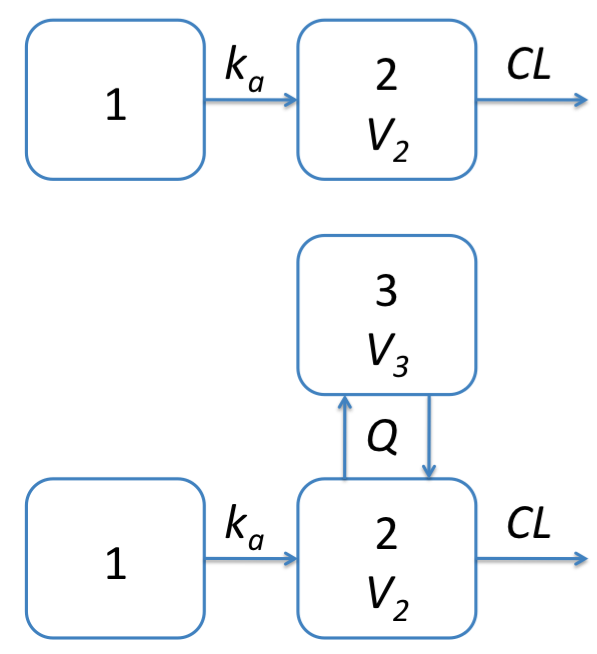
\includegraphics[width=3.5in,trim=0in 0in 0 0in]{graphics/cptModels.png}
\caption{One and two compartment models with first order absorption implemented in Torsten.}
\label{cptModels}
\end{figure}

\texttt{PKModelTwoCpt} can be used to fit example 1, see \texttt{TwoCptModelExample.stan}. Four MCMC chains of 2000 iterations were simulated. The first 1000 iteration of each chain were discarded. Thus 1000 MCMC samples were used for the subsequent analyses.

\begin{figure}
\caption{Stan language for fitting a two compartment model using the \texttt{PKModelTwoCpt} function (abstract)}
\begin{center}
\begin{small}
\begin{fmpage}{\textwidth - .75in}
\begin{lstlisting}[basicstyle=\footnotesize\ttfamily,mathescape=true,flexiblecolumns=true,frame=single,escapeinside=`']
`\bf{data}' {
  int<lower = 1> nt; `\textcolor{gray}{\# number of events}'
  int<lower = 1> nObs; `\textcolor{gray}{\# number of observation}'
  int<lower = 1> iObs[nObs]; `\textcolor{gray}{\# index of observation}'
  int<lower = 1> cmt[nt];
  int evid[nt];
  int addl[nt];
  int ss[nt];
  real amt[nt];
  real time[nt];
  real rate[nt];
  real ii[nt];
  
  vector<lower = 0>[nObs] cObs; `\textcolor{gray}{\#  observed concentration (Dependent Variable)}'
}
                                    $\vdots$ 
`\bf{parameters}' {
  real<lower = 0> CL;
  real<lower = 0> Q;
  real<lower = 0> V2;
  real<lower = 0> V3;
  real<lower = 0> ka;
  real<lower = 0> sigma;
}

`\bf{transformed parameters}' {
                                    $\vdots$ 
  theta[1][1] = CL;
  theta[1][2] = Q;
  theta[1][3] = V2;
  theta[1][4] = V3;
  theta[1][5] = ka;
  theta[1][6] = 1; `\textcolor{gray}{\#  F1}'
  theta[1][7] = 1; `\textcolor{gray}{\#  F2}'
  theta[1][8] = 1; `\textcolor{gray}{\#  F3}'
  theta[1][9] = 0; `\textcolor{gray}{\#  tlag1}'
  theta[1][10] = 0; `\textcolor{gray}{\#  tlag2}'
  theta[1][11] = 0; `\textcolor{gray}{\#  tlag3}'

  x = `\textcolor{red}{PKModelTwoCpt}'(theta, time, amt, rate, ii, evid, cmt, addl, ss);

  cHat = col(x, 2) ./ V2; `\textcolor{gray}{\#  get concentration in the central compartment}'

  for(i in 1:nObs){
    cHatObs[i] = cHat[iObs[i]];`\textcolor{gray}{\# predictions for observed data records}'
  }
 }

`\bf{model}' {
  # priors
  CL ~ lognormal(log(10), 0.25);
  Q ~ lognormal(log(15), 0.5);
  V2 ~ lognormal(log(35), 0.25);
  V3 ~ lognormal(log(105), 0.5);
  ka ~ lognormal(log(2.5), 1);
  sigma ~ cauchy(0, 1);

  logCObs ~ normal(log(cHatObs), sigma);
}                                             
\end{lstlisting}
\end{fmpage}
\end{small}
\end{center}
\label{example1.1Model}
\end{figure}

\textbf{Result.} The MCMC history plots (Figure 3) suggest that the 4 chains have converged to common distributions for all of the key model parameters. The  fit to the plasma concentration data (Figure 5) are in close agreement with the data, which is not surprising since the fitted model is identical to the one used to simulate the data. Similarly the parameter estimates summarized in Table 1 are consistent with the values used for simulation.

\begin{figure}[htbp]
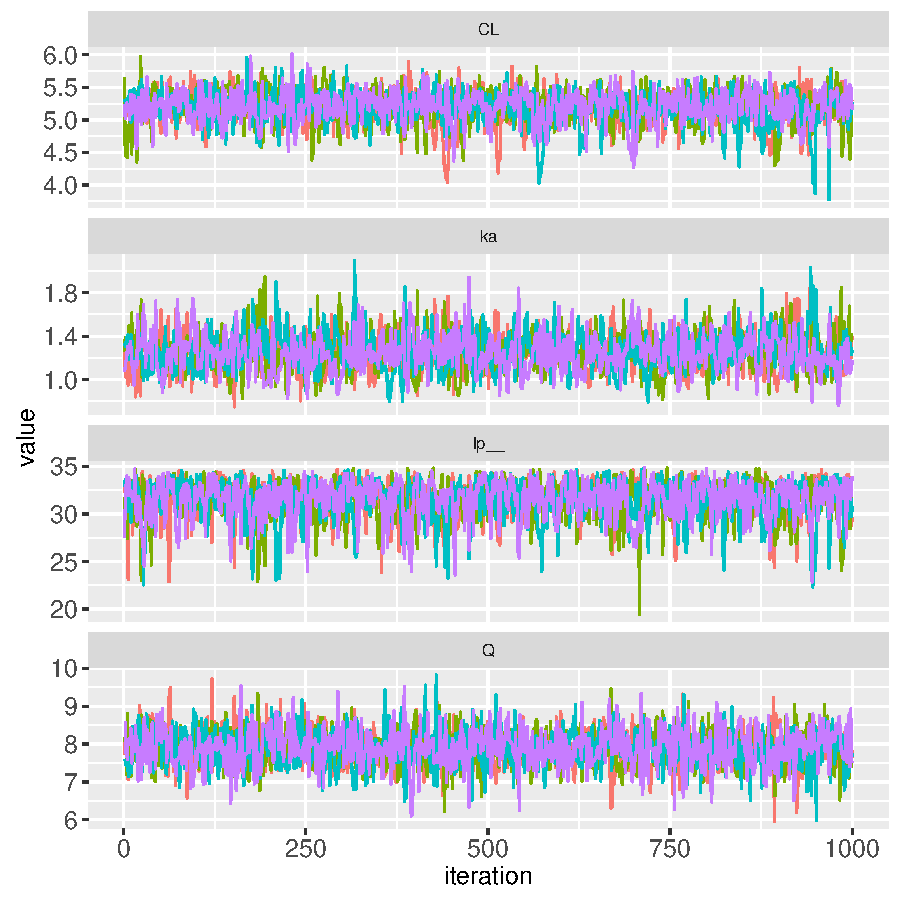
\includegraphics[width=3.0in,trim=0in 0in 0 0in]{graphics/TwoCptModelExamplePlots001.pdf}
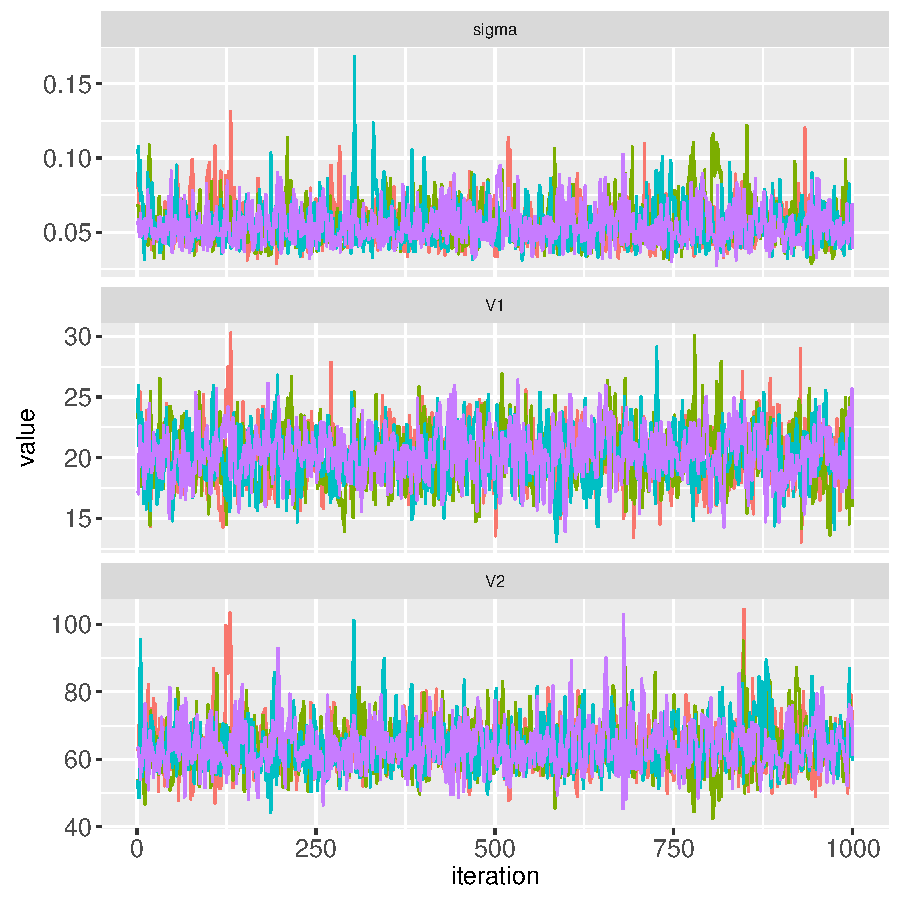
\includegraphics[width=3.0in,trim=0in 0in 0 0in]{graphics/TwoCptModelExamplePlots002.pdf}
\caption{{MCMC history plots for the parameters of a two compartment model with first order absorption (each color corresponds to a different chain)}}
\label{MCMC1}
\end{figure}

\begin{figure}[htbp]
\begin{center}
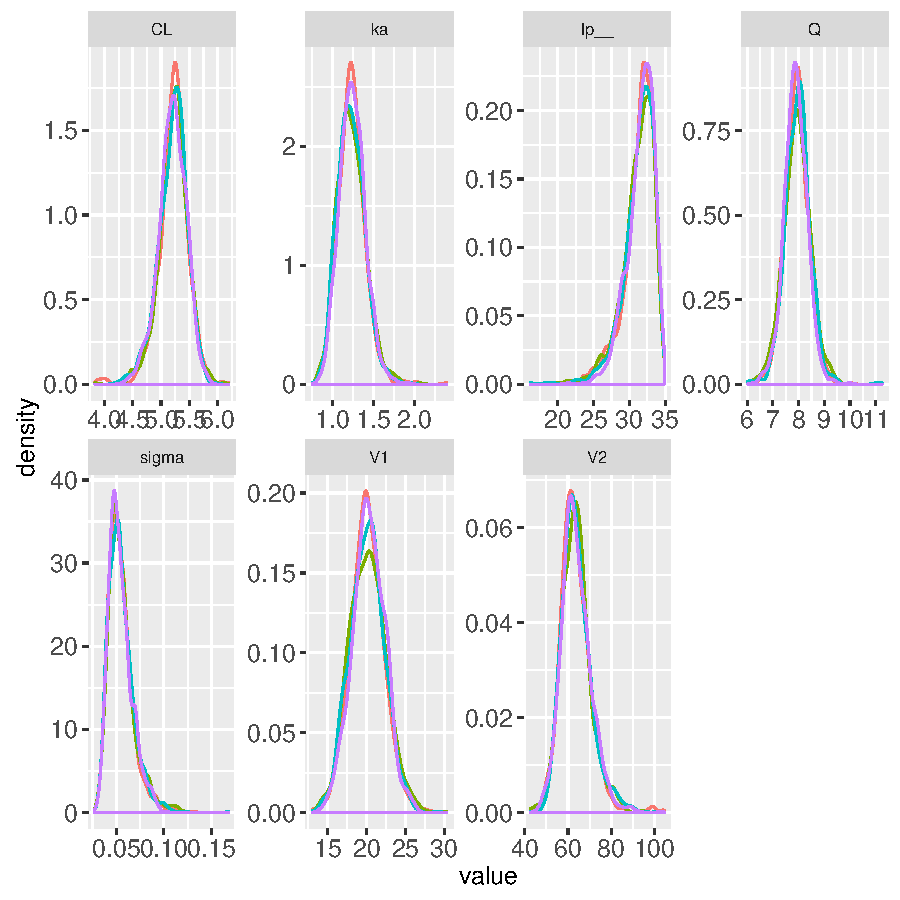
\includegraphics[width=3.5in,trim=0in 0in 0 0in]{graphics/TwoCptModelExamplePlots004.pdf}
\caption{{Posterior Marginal Densities of the Model Parameters (each color corresponds to a different chain)}}
\label{MCMC1}
\end{center}
\end{figure}

\begin{figure}[htbp]
\begin{center}
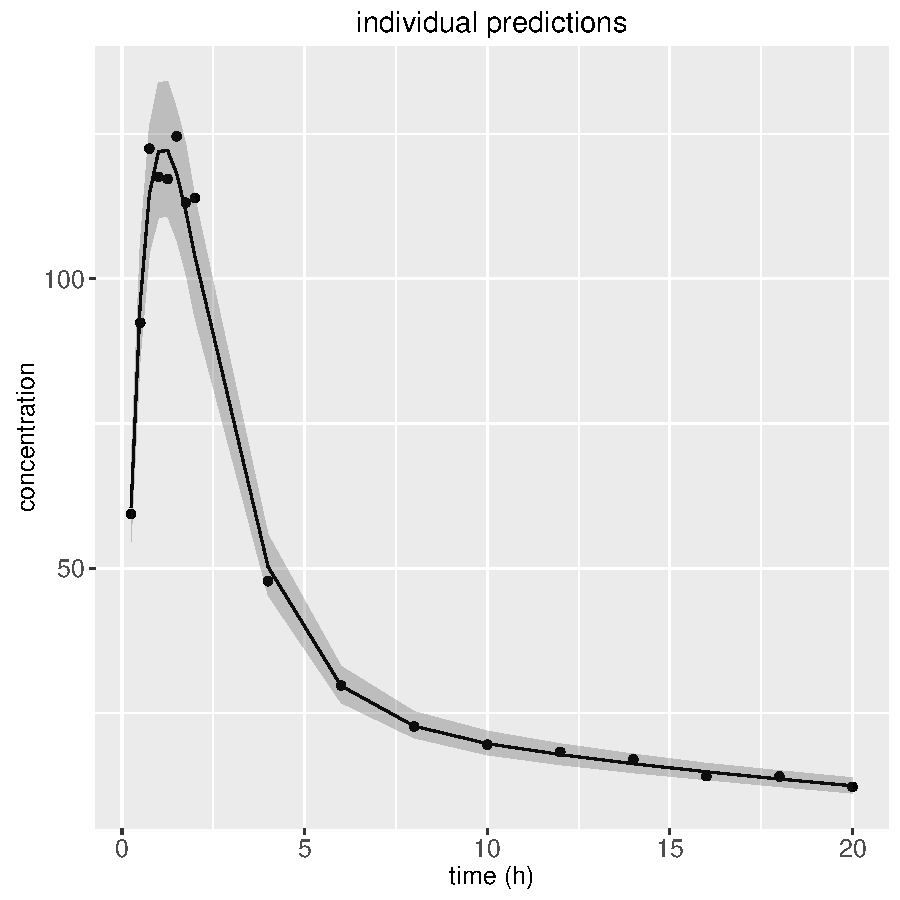
\includegraphics[width=3.5in,trim=0in 0in 0 0in]{graphics/TwoCptModelExamplePlots006.pdf}
\caption{{Predicted (posterior median and 90 \% credible intervals) and observed plasma drug concentrations}}
\label{predictions}
\end{center}
\end{figure}

\begin{table}[ht]
\centering
\caption{Summary of the MCMC simulations of the marginal posterior distributions of the model parameters}
\begin{tabular}{rrrrrrrrrrr}
  \hline
 & mean & se\_mean & sd & 2.5\% & 25\% & 50\% & 75\% & 97.5\% & n\_eff & Rhat \\ 
  \hline
CL & 5.19 & 0.01 & 0.25 & 4.60 & 5.05 & 5.21 & 5.35 & 5.62 & 971.04 & 1.00 \\ 
  Q & 7.90 & 0.01 & 0.47 & 6.97 & 7.58 & 7.93 & 8.21 & 8.79 & 1662.02 & 1.00 \\ 
  V2 & 20.25 & 0.08 & 2.27 & 15.71 & 18.74 & 20.23 & 21.76 & 24.67 & 896.67 & 1.00 \\ 
  V3 & 64.10 & 0.22 & 6.98 & 52.60 & 59.48 & 63.38 & 67.74 & 80.65 & 1032.66 & 1.00 \\ 
  ka & 1.25 & 0.00 & 0.17 & 0.94 & 1.13 & 1.24 & 1.35 & 1.62 & 940.99 & 1.00 \\ 
   \hline
\end{tabular}
\end{table}

\subsection*{General Linear Compartment Model}
A general linear compartment model refers to a model that may be described in terms of a system of first order linear differential equations with (piecewise) constant coefficients, i.e., a differential equation of the form:
$$ x^\prime\left(t\right) = Kx\left(t\right) $$
where $K$ is a matrix. For example $K$ for a two compartment model with first order absorption is:
$$   K = \left[\begin{array}{ccc}
	-k_a & 0 & 0 \\
	k_a & -\left(k_{10} + k_{12}\right) & k_{21} \\
	0 & k_{12} & -k_{21}
	\end{array}\right] $$ \\
where $k_{10} = CL / V2 $, $ k_{12} = Q / V2 $, and $k_{21} = Q / V2 $.

The linear compartment model has the form:

\texttt{linCptModel(K, theta, time, amt, rate, ii, evid, cmt, addl, ss)}

where \texttt{K} is the matrix describing the ODE system. Since most of the parameters appear in \texttt{K}, it is not necessary to specify them again in \texttt{theta}. Instead, we only specify in \texttt{theta} parameters left out of \texttt{K}, namely the bioavailability fractions and the lag times.

\begin{figure}
\caption{Stan language for fitting a two compartment model using the \texttt{linCptModel} function (abstract)}
\begin{center}
\begin{small}
\begin{fmpage}{\textwidth - .75in}
\begin{lstlisting}[basicstyle=\footnotesize\ttfamily,mathescape=true,flexiblecolumns=true,frame=single,escapeinside=`']
`\bf{transformed parameters}' {
  `\textcolor{red}{matrix[3, 3] K;}'
  real k10;
  real k12;
  real k21;
  vector<lower = 0>[nTheta] theta[1];
  vector<lower = 0>[nt] cHat;
  vector<lower = 0>[nObs] cHatObs;
  matrix<lower = 0>[nt, 3] x;
  
  k10 = CL / V2;
  k12 = Q / V2;
  k21 = Q / V3;
 
  `\textcolor{red}{K = rep\_matrix(0, 3, 3);}'

  `\textcolor{red}{K[1, 1] = -ka;}'  
  `\textcolor{red}{K[2, 1] = ka;}' 
  `\textcolor{red}{K[2, 2] = -(k10 + k12);}' 
  `\textcolor{red}{K[2, 3] = k21;}' 
  `\textcolor{red}{K[3, 2] = k12;}' 
  `\textcolor{red}{K[3, 3] = -k21;}'

  theta[1][1] = 1; # F1
  theta[1][2] = 1; # F2
  theta[1][3] = 1; # F3
  theta[1][4] = 0; # tlag1
  theta[1][5] = 0; # tlag2
  theta[1][6] = 0; # tlag3

  x = `\textcolor{red}{linCptModel}'(`\textcolor{red}{K}', theta, time, amt, rate, ii, evid, cmt, addl, ss);

  cHat = col(x, 2) ./ V1;

  for(i in 1:nObs){
    cHatObs[i] = cHat[iObs[i]]; `\textcolor{gray}{\# predictions for observed data records}'
  }
}

`\bf{model}'{
  logCObs ~ normal(log(cHatObs), sigma);
}
\end{lstlisting}
\end{fmpage}
\end{small}
\end{center}
\label{example1.1Model}
\end{figure}

\subsection*{General Compartment Model}

Torsten may be used to fit models described by a system of first-order ODE's, i.e., differential equations of the form:
$$ x^\prime\left(t\right) = f\left(t, x\left(t\right)\right) $$
where $x$ and $f$ are vector-valued functions.

The general compartment model functions have the form:

\texttt{<model\_name>(ODE\_system, nCmt, \\
                              theta, time, amt, rate, ii, evid, cmt, addl, ss, \\
                              rel\_tol, abs\_tol, max\_step)}
                              
where \texttt{ODE\_system} is a system of first-order ODE's defined in the function block of Stan (see section 19.2 of the Stan reference manual) and \texttt{nCmt} is the number of compartments in the model. \texttt{rel\_tol}, \texttt{abs\_tol}, and \texttt{max\_step} are the tuning parameters for the ODE integrator, respectively the relative tolerance, the absolute tolerance, and the maximum number of steps. It is difficult to recommend values for the tuning parameters, though the authors typically use $rel\_tol = 1e-8$, $abs\_tol = 1e-8$ and $max\_step = 1e+8$. For more details see Stan's reference manual.

The options for \texttt{model\_name} are:
\begin{itemize}
  \item generalCptModel\_rk45
  \item generalCptModel\_CVODES
\end{itemize}

They respectively call the built-in Runge-Kutta 4th/5th integrator, recommended for non-stiff ODE's, and CVODES integrator, recommended for stiff ODE's.

\begin{figure}
\caption{Stan language for fitting a two compartment model using the \texttt{genCptModel\_rk45} function (abstract)}
\begin{center}
\begin{small}
\begin{fmpage}{\textwidth - .75in}
\begin{lstlisting}[basicstyle=\footnotesize\ttfamily,mathescape=true,flexiblecolumns=true,frame=single,escapeinside=`']
`\bf{functions}'{
  # define ODE system for two compartment model
  real[] `\textcolor{red}{twoCptModelODE}'(real t,
			       real[] x,
			       real[] theta,
			       real[] rate, # in this example, rate is treated as data
			       int[] dummy){
    real Q;
    real CL;
    real V1;
    real V2;
    real ka;
    real k12;
    real k21;
    real k10;
    real y[3]; 
    
    CL = theta[1];
    Q = theta[2];
    V1 = theta[3];
    V2 = theta[4];
    ka = theta[5];
    k10 = CL / V1;
    k12 = Q / V1;
    k21 = Q / V2;

    y[1] = -ka*x[1];
    y[2] = ka*x[1] - (k10 + k12)*x[2] + k21*x[3];
    y[3] = k12*x[2] - k21*x[3];

    return y;
  }
}
                                    $\vdots$
`\bf{transformed parameters}' {
                                    $\vdots$
  theta[1][1] = CL;
  theta[1][2] = Q;
  theta[1][3] = V1;
  theta[1][4] = V2;
  theta[1][5] = ka;
  theta[1][6] = 1; # F1
  theta[1][7] = 1; # F2
  theta[1][8] = 1; # F3
  theta[1][9] = 0; # tlag1
  theta[1][10] = 0; # tlag2
  theta[1][11] = 0; # tlag3

  x = `\textcolor{red}{generalCptModel\_bdf}'( `\textcolor{red}{twoCptModelODE}', 3,
                          theta, time, amt, rate, ii, evid, cmt, addl, ss,
                          1e-8, 1e-8, 1e8);
                                    $\vdots$
\end{lstlisting}
\end{fmpage}
\end{small}
\end{center}
\label{example1.1Model}
\end{figure}

\subsection*{Summary}

\begin{table} %[htdp]
\caption{Arguments of Torsten functions.}
\begin{center}
\begin{minipage}{\textwidth - 1in}
\begin{tabular}{p{1.5in}cp{1.5in}p{1.5in}} 
\hline\hline
 & & & model \\
 & function & argument & parameters \\
model & name & names & in {\tt theta} \\ 
\hline
{\raggedright one compartment\\ model with first order\\ absorption
  $\left(k_a > \frac{CL}{V_2}\right)$} & {\tt PKModelOneCpt} &  
	{\tt time}, {\tt amt}, {\tt rate}, {\tt ii}, {\tt evid}, {\tt cmt}, {\tt addl}, {\tt ss} &
	$CL$, $V_2$, $k_a$, $F_1$, $F_2$, $t_{lag1}$, $t_{lag2}$ \\
\hline
{\raggedright two compartment\\ model with first order\\ absorption $\left(k_a > \lambda_1\footnote{
	$\lambda_1 = \frac{k_{10}+k_{12}+k_{21} - \sqrt{\left(k_{10}+k_{12}+k_{21}\right)^2 - 4k_{10}k_{21}}}{2}$ where $k_{10} = \frac{CL}{V_2}$,
	$k_{12} = \frac{Q}{V_2}$ and $k_{21} = \frac{Q}{V_3}$.}\right)$} & {\tt PKModelTwoCpt} &  
	{\tt time}, {\tt amt}, {\tt rate}, {\tt ii}, {\tt evid}, {\tt cmt}, {\tt addl}, {\tt ss} &
	$CL$, $Q$, $V_2$, $V_3$, $k_a$,
	$F_1$, $F_2$, $F_3$, $t_{lag1}$, $t_{lag2}$, $t_{lag2}$ \\ 
\hline
{\raggedright general linear \\ compartment model} & {\tt linCptModel} &  
	{\tt K}, {\tt time}, {\tt amt}, {\tt rate}, {\tt ii}, {\tt evid}, {\tt cmt}, {\tt addl}, {\tt ss} &
	$F_1$ to $F_n$, $t_{lag1}$ to $t_{lagn}$ \\
\hline
{\raggedright general compartment \\ models} & {\tt genCptModel\_*} &  
	{\tt ODE\_system}, {\tt nCmt}, {\tt time}, {\tt amt}, {\tt rate}, {\tt ii}, {\tt evid},
        {\tt cmt}, {\tt addl}, {\tt ss}, {\tt rel\_tol}, {\tt abs\_tol}, {\tt max\_num\_steps}  &
	Parameters in ODE system, $F_1$ to $F_n$, $t_{lag1}$ to $t_{lagn}$
\end{tabular}
\end{minipage}
\end{center}
\label{precompiledModels}
\end{table}

Table 2 summarizes how to call Torsten functions.

It is key thing to understand which type of models each function works for, and which method optimizes model fitting. A analytical method will always be fastest, but only applies to a few simple cases. Numerical methods that use an ODE integrator are generally applicable, but are orders of magnitude slower. The matrix exponential solutions falls, speed-wise, between the analytical and the numerical solution, and can be used for all linear ODE's system. 


\section{Additional Example}

\subsection*{Example 2: Effect Compartment Model}
We now expand example 1 to a population model fitted to the combined data from phase I and phase IIa studies. The parameters exhibit inter-individual variations (IIV), due to both random effects and to the patients' body weight, treated as a covariate and denoted $bw$:

\subsubsection*{Population Model for Plasma Drug Concentration ($c$)}
\begin{eqnarray*}
 \log\left(c_{ij}\right) &\sim& N\left(\log\left(\widehat{c}_{ij}\right),\sigma^2\right) \\
 \widehat{c}_{ij} &=& f_{2cpt}\left(t_{ij},D_j,\tau_j,CL_j,Q_j,V_{1j},V_{2j},k_{aj}\right) \\
 \log\left(CL_j,Q_j,V_{ssj},k_{aj}\right) &\sim&
   \lefteqn{N\left(\log\left(\widehat{CL}\left(\frac{bw_j}{70}\right)^{0.75},\widehat{Q}\left(\frac{bw_j}{70}\right)^{0.75},
	\widehat{V}_{ss}\left(\frac{bw_j}{70}\right),\widehat{k}_a\right),\Omega\right)} \\
 V_{1j} &=& f_{V_1}V_{ssj} \ \ \ \ \ \ V_{2j} = \left(1 - f_{V_1}\right)V_{ssj} \\
 \left(\widehat{CL},\widehat{Q},\widehat{V}_{ss},\widehat{k}_a, f_{V_1}\right) &=& 
	\left(10\ {\rm L/h},15\  {\rm L/h},140\  {\rm L},2\ {\rm h^{-1}}, 0.25 \right) \\
\Omega &=& \left(\begin{array}{cccc} 0.25^2 & 0 & 0 & 0 \\ 0 & 0.25^2 & 0 & 0 \\
0 & 0 & 0.25^2 & 0 \\ 0 & 0 & 0 & 0.25^2  \end{array}\right), \ \ \ \sigma = 0.1 \\
\end{eqnarray*}

Furthermore we add a fourth compartment in which we measure a PD effect (see figure 8).

\begin{figure}[htbp]
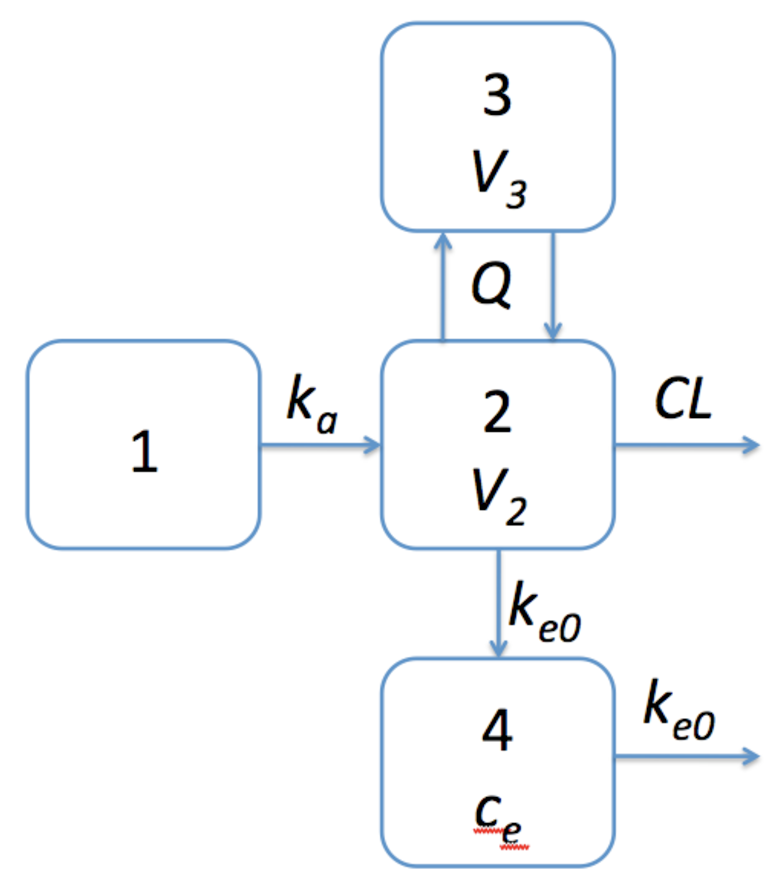
\includegraphics[width=3.5in,trim=0in 0in 0 0in]{graphics/effectCptModel.pdf}
\caption{Effect Compartment Model}
\label{effCptModel}
\end{figure}

\subsubsection*{Effect Compartment Model for PD response ($R$)}
\begin{eqnarray*}
R_{1ij} &\sim& N\left(\widehat{R}_{ij},\sigma_{R}^2\right) \\
\widehat{R}_{ij} &=& \frac{E_{max}c_{eij}}{EC_{50j} + c_{eij}} \\
c_{e\cdot j}^\prime &=& k_{e0j}\left(c_{\cdot j} - c_{e\cdot j}\right) \\
\log\left(EC_{50j}, k_{e0j}\right) &\sim& N\left(\log\left(\widehat{EC}_{50}, \widehat{k}_{e0}\right),\Omega_R\right) \\
\left(E_{max}, \widehat{EC}_{50},\widehat{k}_{e0}\right) &=& \left(100, 100.7, 1\right) \\
\Omega_R &=& \left(\begin{array}{cc} 0.2^2 & 0 \\ 0 & 0.25^2  \end{array}\right), \ \ \ \sigma_R = 10
\end{eqnarray*}

The PK and the PD data are simulated using the following treatment.
\begin{itemize}
  \item Phase I study
  \begin{itemize}
    \item Single dose and multiple doses
    \item Parallel dose escalation design
    \item 25 subjects per dose
    \item Single doses: 1.25 
    \item PK: plasma concentration of parent drug ($c$)
    \item PD response: Emax function of effect compartment concentration ($R$)
    \item PK and PD measured at 0.083, 0.167, 0.25, 0.5, 0.75, 1, 2, 3, 4, 6, 8, 12, 18, and 24 hours
  \end{itemize}
  \item Phase IIa trial in patients
  \begin{itemize}
    \item 100 subjects
    \item Multiple doses: 20 mg
    \item sparse PK and PD data (3-6 samples per patient)
  \end{itemize}
\end{itemize}

The model is now simultaneously fitted to the PK and the PD data! For this four compartment model, we construct a constant rate matrix and use \texttt{linCptModel}. Correct use of Torsten requires that the user pass the entire event history (observation and dosing events) for an individual to the function. Thus the Stan model shows the call to \texttt{linCptModel} within a loop over the individual subjects rather than over the individual observations.

\begin{figure}
\caption{Stan language for fitting an effect compartment model using \texttt{linCptModel} (abstract)}
\begin{tiny}
\begin{center}
\begin{fmpage}{\textwidth - .75in}
\begin{lstlisting}[basicstyle=\tiny\ttfamily,mathescape=true,flexiblecolumns=true,frame=single,escapeinside=`']
transformed parameters {
  for(j in 1:nSubjects){
                             $\vdots$
  Omega = quad_form_diag(rho, omega);

  for(j in 1:nSubjects){
    CL[j] = exp(logtheta[j, 1]) * (weight[j] / 70)^0.75;
    Q[j] = exp(logtheta[j, 2]) * (weight[j] / 70)^0.75;
    V1[j] = exp(logtheta[j, 3]) * weight[j] / 70;
    V2[j] = exp(logtheta[j, 4]) * weight[j] / 70;
    ka[j] = exp(logtheta[j, 5]);
    ke0[j] = exp(logKe0[j]);
    EC50[j] = exp(logEC50[j]);

    k10 = CL[j] / V1[j];
    k12 = Q[j] / V1[j];
    k21 = Q[j] / V2[j];

    K = rep_matrix(0, 4, 4);
    K[1, 1] = -ka[j];
    K[2, 1] = ka[j];
    K[2, 2] = -(k10 + k12);
    K[2, 3] = k21;
    K[3, 2] = k12;
    K[3, 3] = -k21;
    K[4, 2] = ke0[j];
    K[4, 4] = -ke0[j];
                        
    ke0[j] = exp(logKe0[j]);
    EC50[j] = exp(logEC50[j]);
    
    k10 = CL[j] / V1[j];
    k12 = Q[j] / V1[j];
    k21 = Q[j] / V2[j];

    K = rep_matrix(0, 4, 4);
    
    K[1, 1] = -ka[j];
    K[2, 1] = ka[j];
    K[2, 2] = -(k10 + k12);
    K[2, 3] = k21;
    K[3, 2] = k12;
    K[3, 3] = -k21;
    K[4, 2] = ke0[j];
    K[4, 4] = -ke0[j];
           
    x[start[j]:end[j],] = `\textcolor{red}{linCptModel}'(K, parms, time[start[j]:end[j]], 
                                        amt[start[j]:end[j]], rate[start[j]:end[j]],
                                        ii[start[j]:end[j]], evid[start[j]:end[j]],
                                        cmt[start[j]:end[j]], addl[start[j]:end[j]], 
                                        ss[start[j]:end[j]]);

    cHat[start[j]:end[j]] = 1000 * x[start[j]:end[j], 2] ./ V1[j];
    ceHat[start[j]:end[j]] = 1000 * x[start[j]:end[j], 4] ./ V1[j];
    respHat[start[j]:end[j]] = 100 * ceHat[start[j]:end[j]] ./ 
       (EC50[j] + ceHat[start[j]:end[j]]);
  }

  for(i in 1:nObs){
    cHatObs[i] = cHat[iObs[i]];
    respHatObs[i] = respHat[iObs[i]];
  }
}
                             $\vdots$  
} 
\end{lstlisting}
\end{fmpage}
\end{center}
\end{tiny} 
\label{example3Model}
\end{figure}

\subsubsection*{Results} We use the same diagnosis tools as for the previous examples. The MCMC history plots (Figure 10) suggest the 4 chains have converge to common distributions. We note some minor auto-correlations for $lp\_$ (the log posterior) and for IIV parameters: specifically $\Omega_{ke\_0}$ and $\rho$. The correlation matrix $\rho$ does not explicitly appear in the model, but it is used to construct $\Omega$, which parametrizes the PK IIV. The fits to the plasma concentration data (Figure 12) are in close agreement with the data, notably for the sparse data case (phase IIa study). The fits to the PD data (figure 13) look good, though the data is more noisy. The model reflects the noise by producing larger confidence intervals. The estimated values of the parameters are consistent with the values used to simulate the data. 

\begin{figure}[htbp]
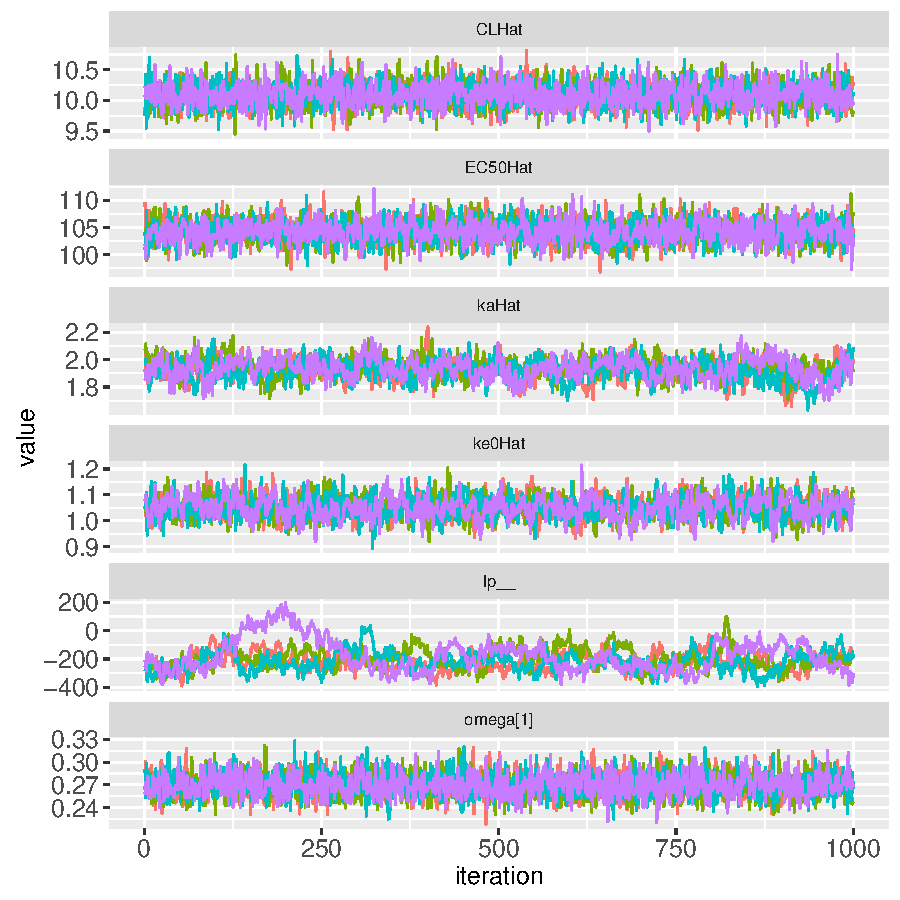
\includegraphics[width=3.0in,trim=0in 0in 0 0in]{graphics/effCptModelTorsten/effCptModelTorstenPlots001.pdf}
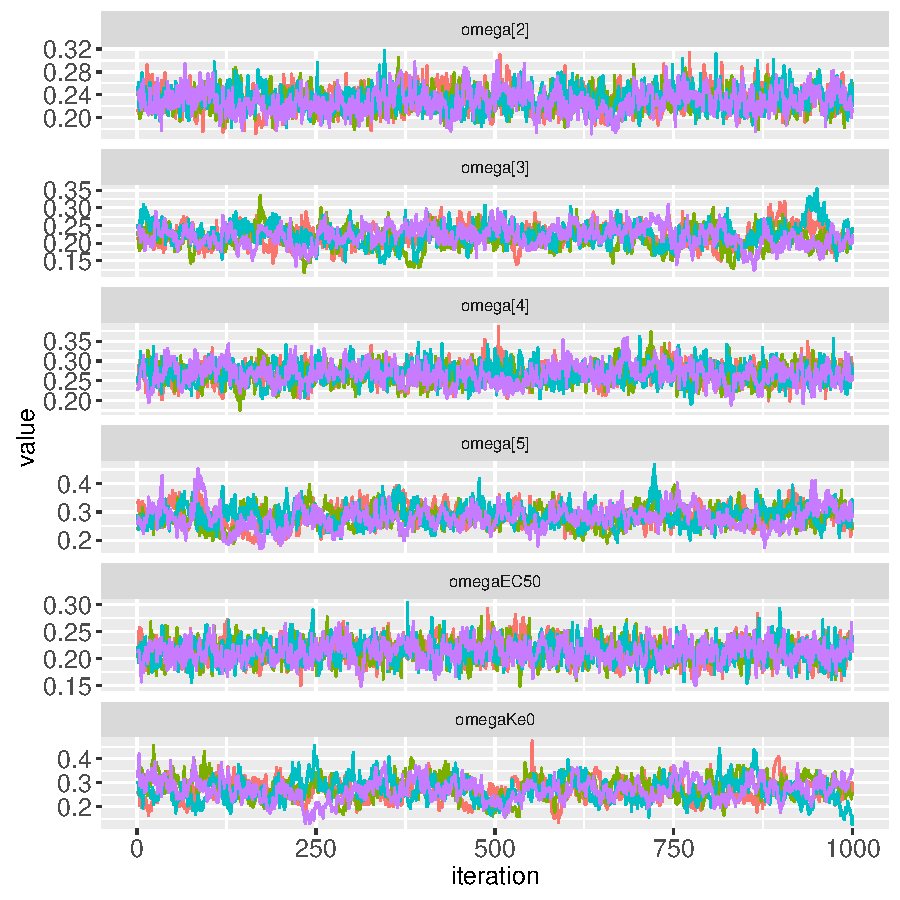
\includegraphics[width=3.0in,trim=0in 0in 0 0in]{graphics/effCptModelTorsten/effCptModelTorstenPlots002.pdf}
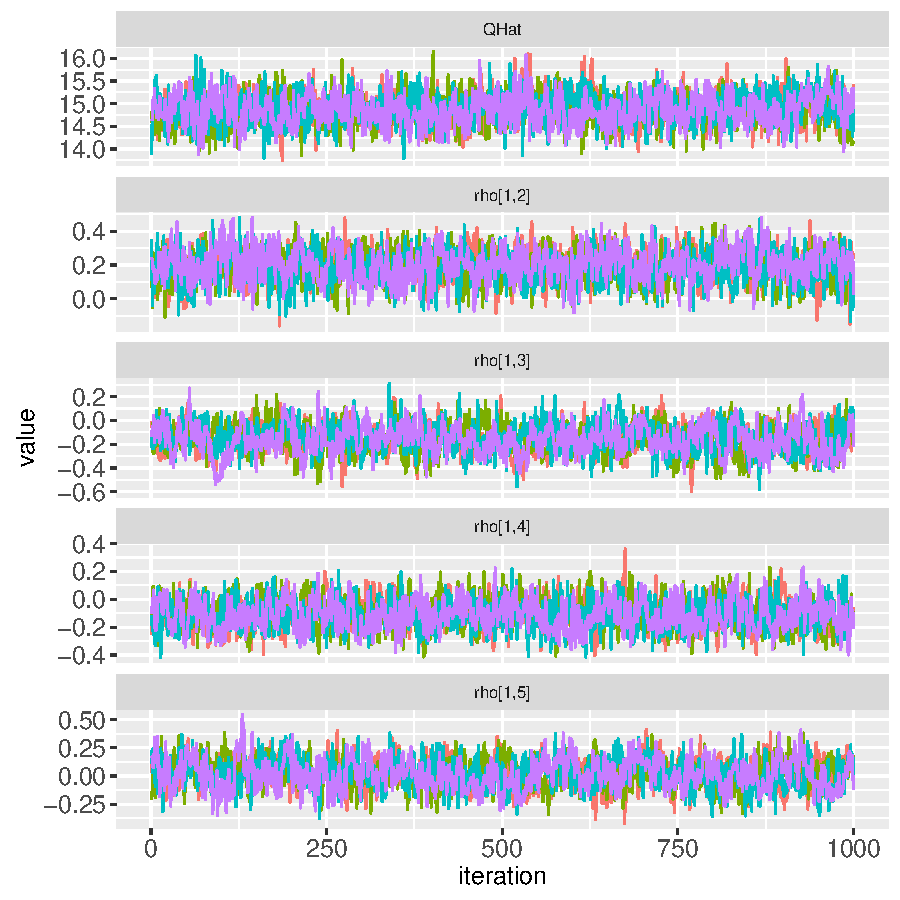
\includegraphics[width=3.0in,trim=0in 0in 0 0in]{graphics/effCptModelTorsten/effCptModelTorstenPlots003.pdf}
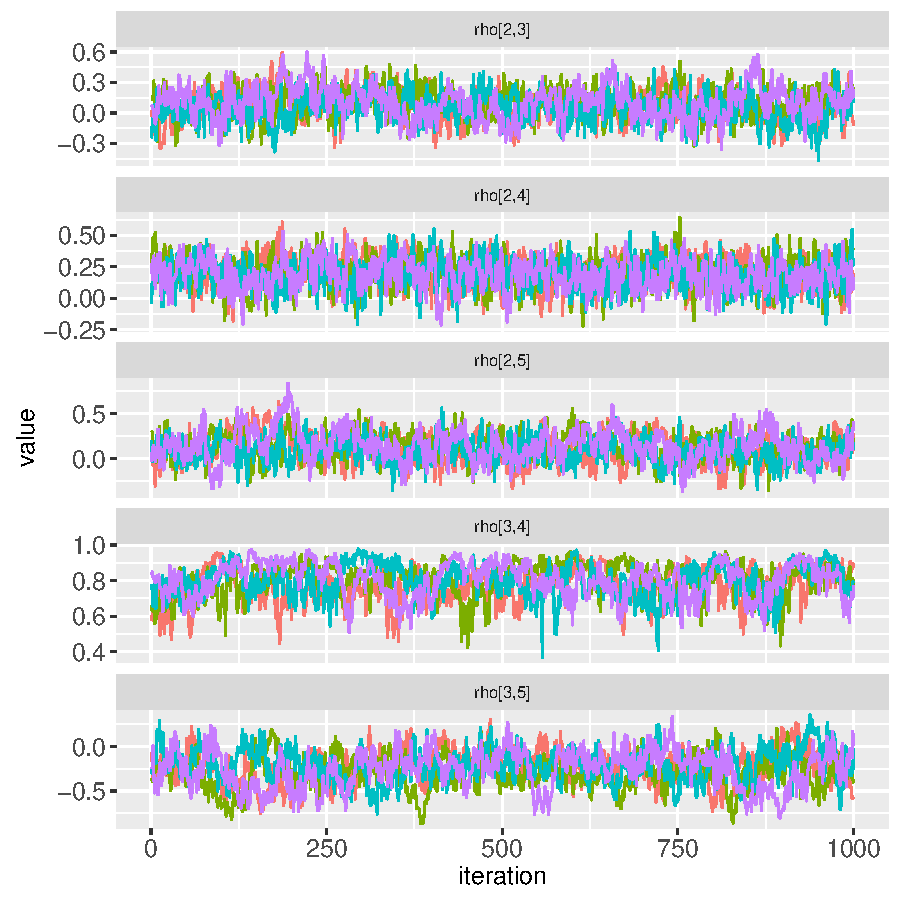
\includegraphics[width=3.0in,trim=0in 0in 0 0in]{graphics/effCptModelTorsten/effCptModelTorstenPlots004.pdf}
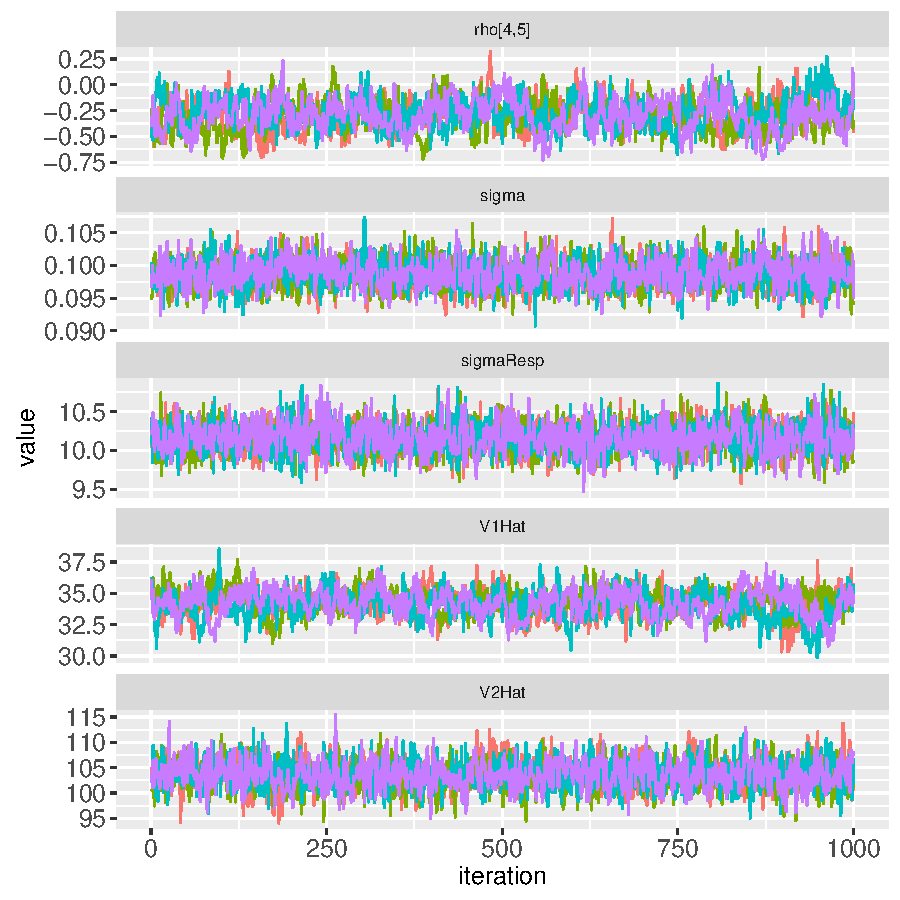
\includegraphics[width=3.0in,trim=0in 0in 0 0in]{graphics/effCptModelTorsten/effCptModelTorstenPlots005.pdf}
\caption{{MCMC history plots for the parameters of a two compartment model with first order absorption (each color corresponds to a different chain)}}
\label{MCMC1}
\end{figure}

\begin{figure}[htbp]
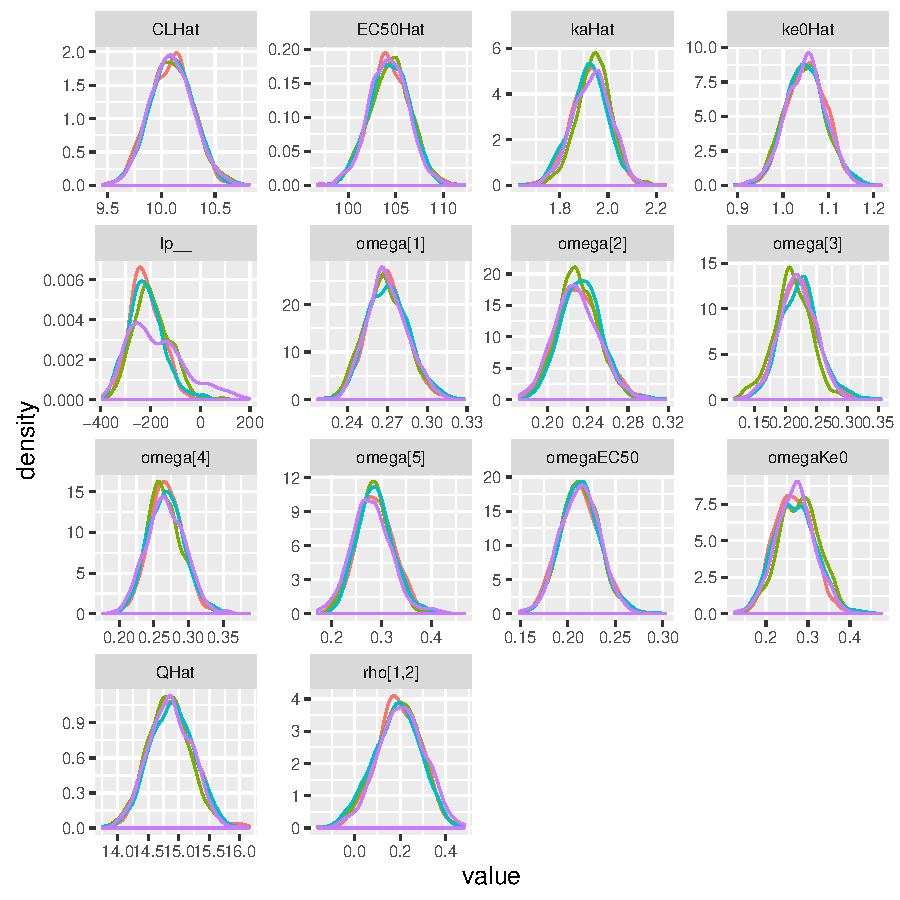
\includegraphics[width=3.0in,trim=0in 0in 0 0in]{graphics/effCptModelTorsten/effCptModelTorstenPlots006.pdf}
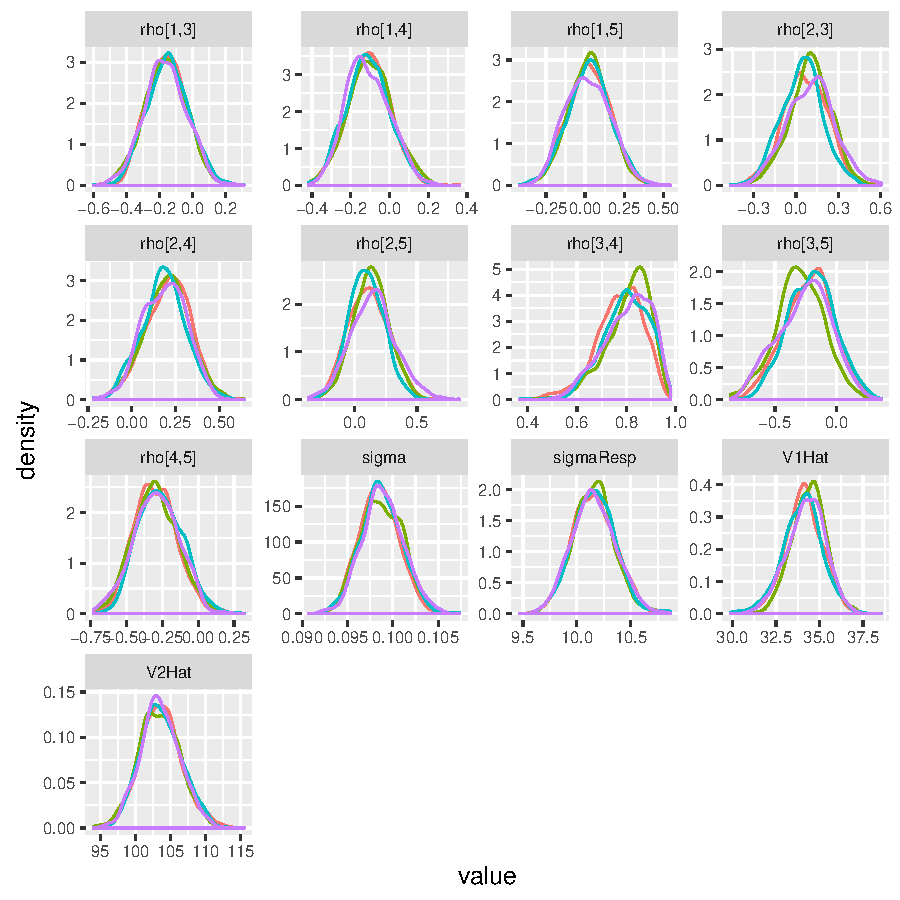
\includegraphics[width=3.0in,trim=0in 0in 0 0in]{graphics/effCptModelTorsten/effCptModelTorstenPlots007.pdf}
\caption{{Posterior Marginal Densities of the Model Parameters (each color corresponds to a different chain)}}
\label{MCMC1}
\end{figure}

\begin{figure}[htbp]
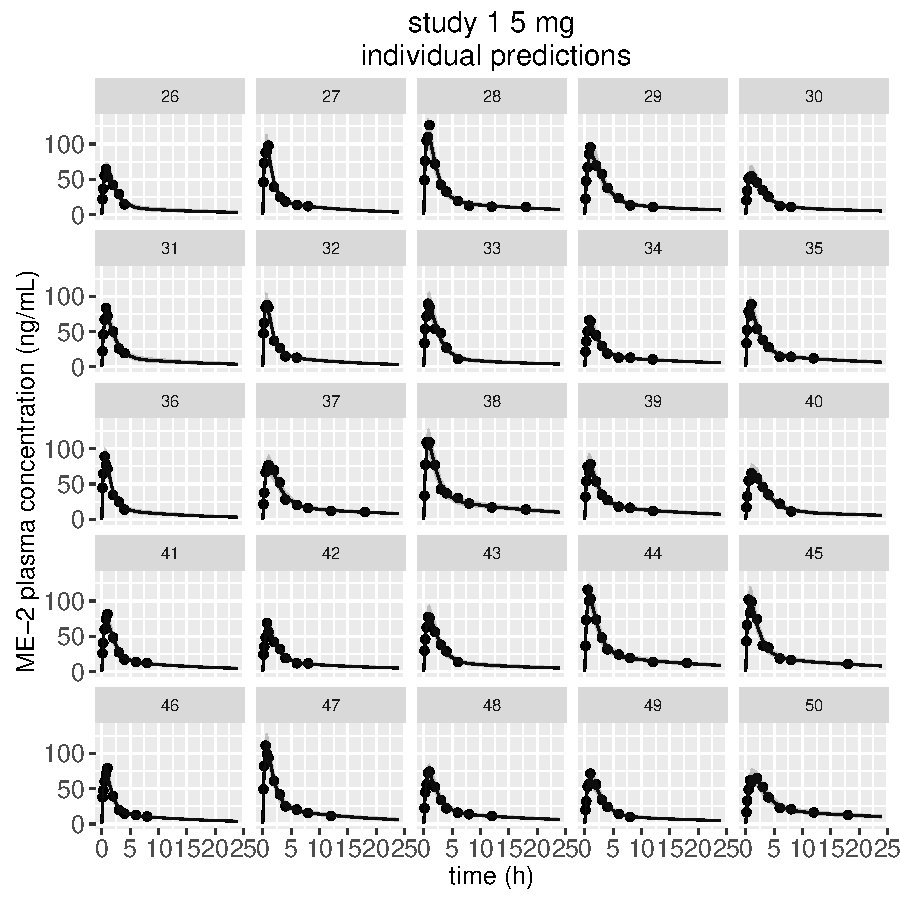
\includegraphics[width=1.5in,trim=0in 0in 0 0in]{graphics/effCptModelTorsten/effCptModelTorstenPlots011.pdf}
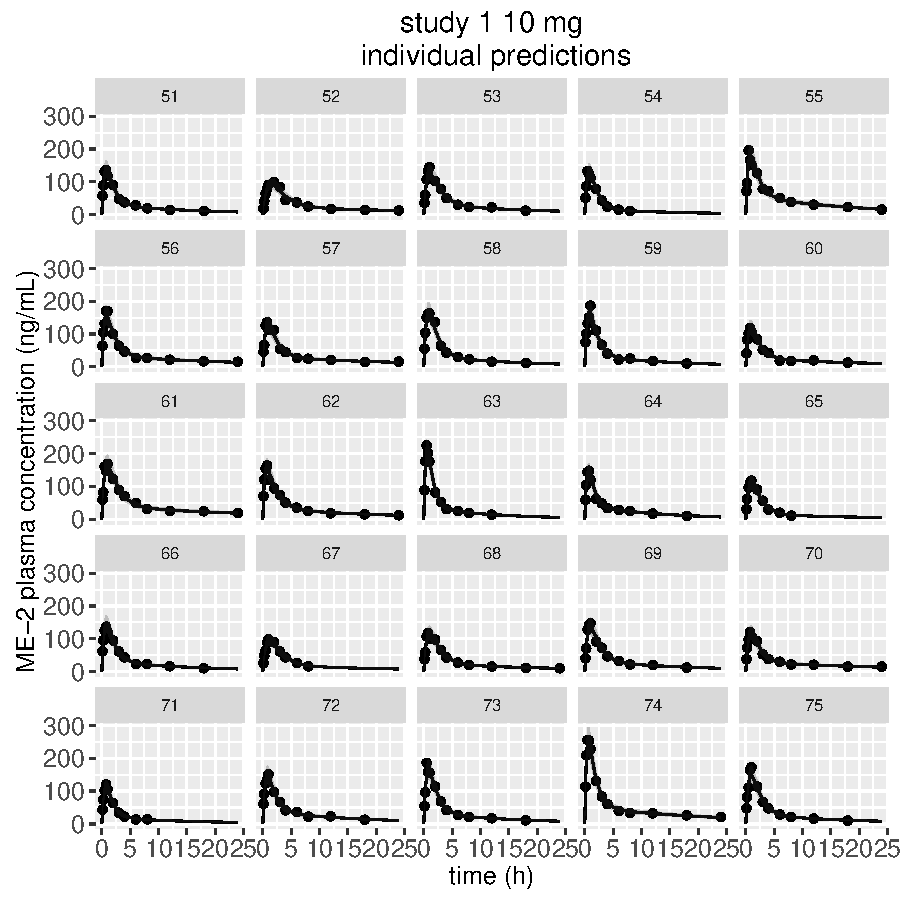
\includegraphics[width=1.5in,trim=0in 0in 0 0in]{graphics/effCptModelTorsten/effCptModelTorstenPlots012.pdf}
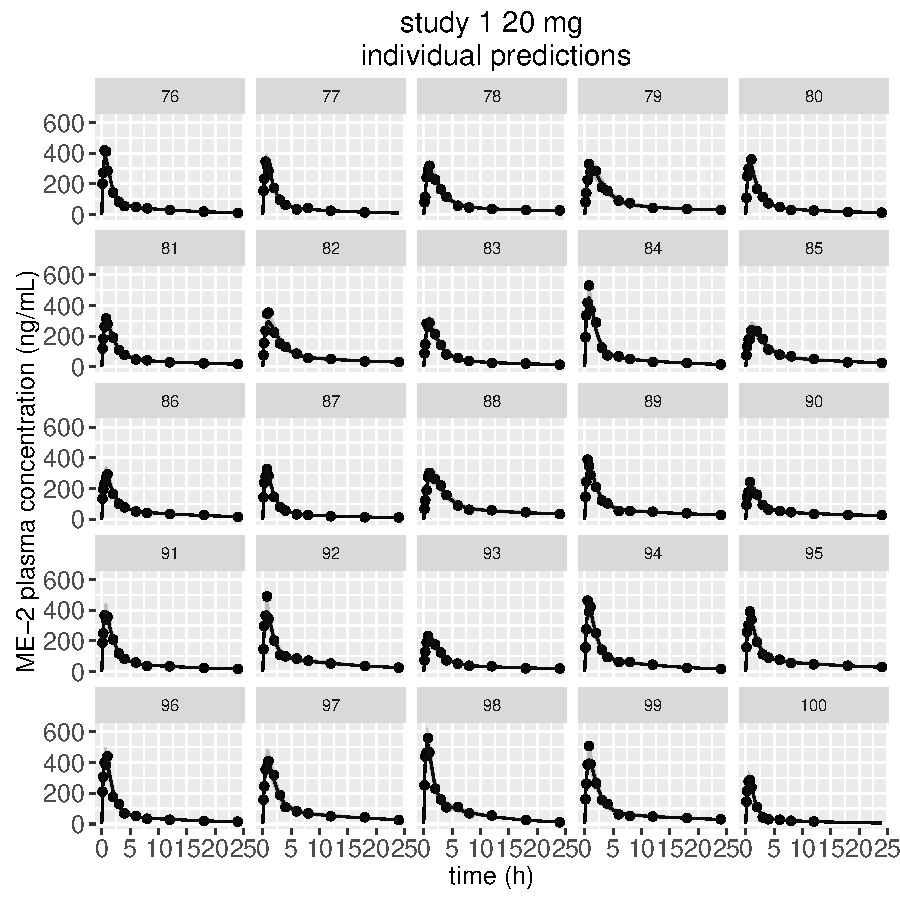
\includegraphics[width=1.5in,trim=0in 0in 0 0in]{graphics/effCptModelTorsten/effCptModelTorstenPlots013.pdf}
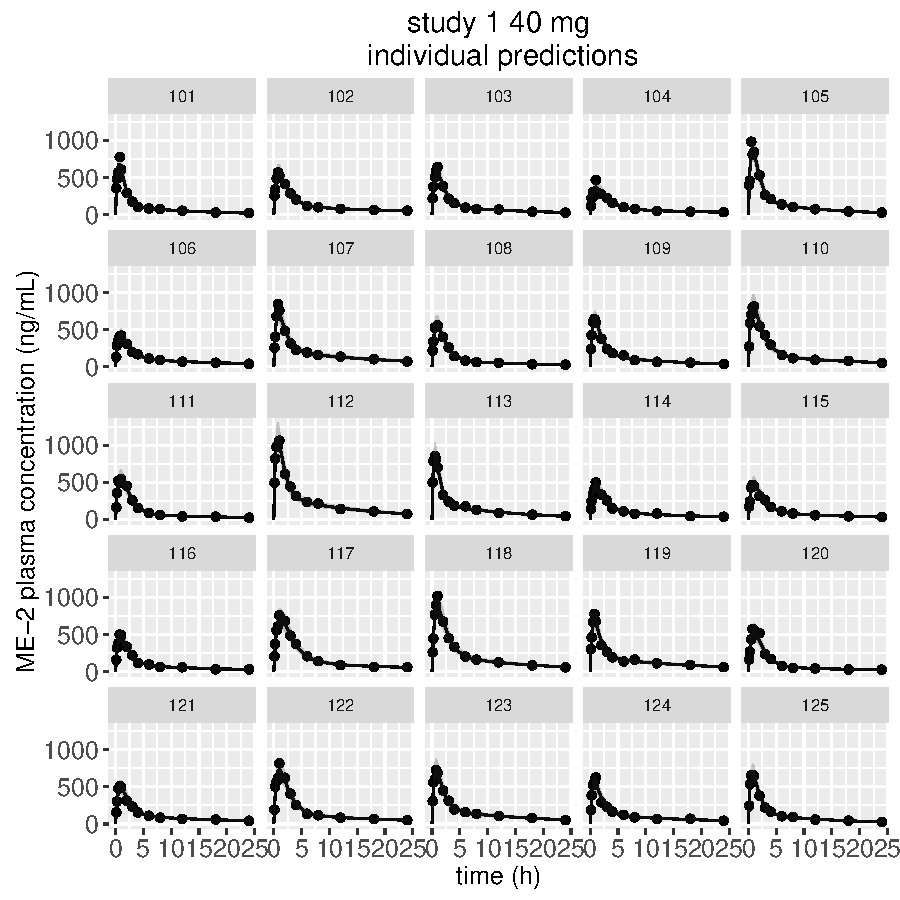
\includegraphics[width=1.5in,trim=0in 0in 0 0in]{graphics/effCptModelTorsten/effCptModelTorstenPlots014.pdf}
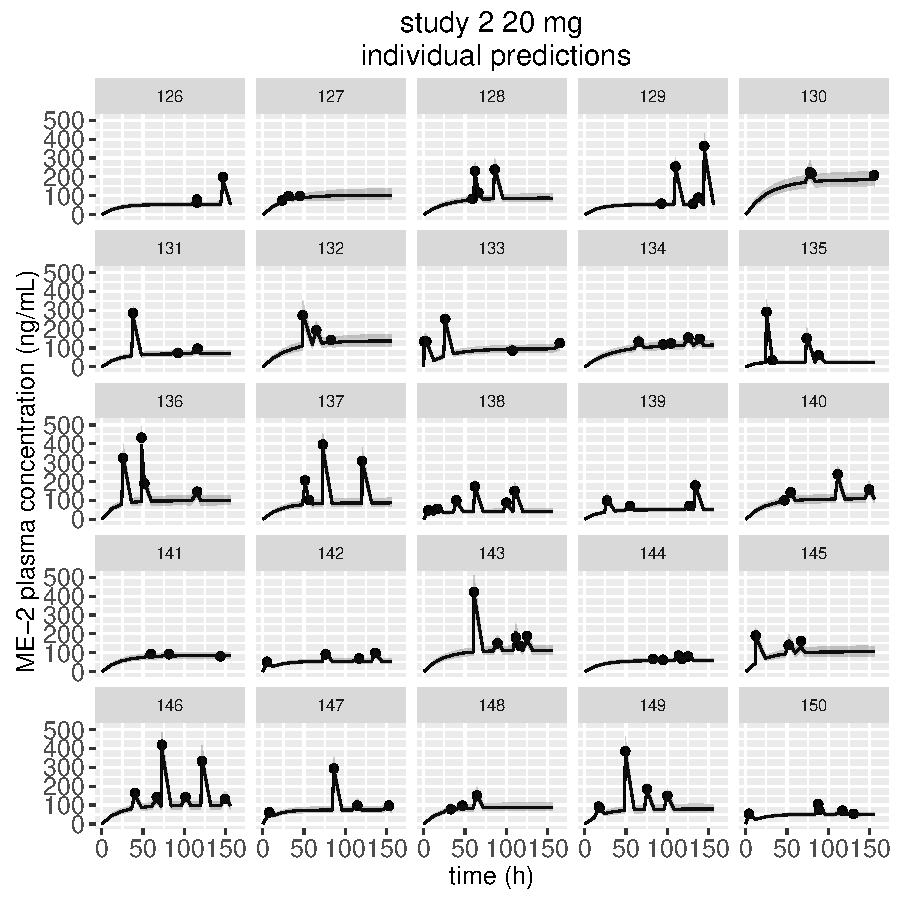
\includegraphics[width=1.5in,trim=0in 0in 0 0in]{graphics/effCptModelTorsten/effCptModelTorstenPlots015.pdf}
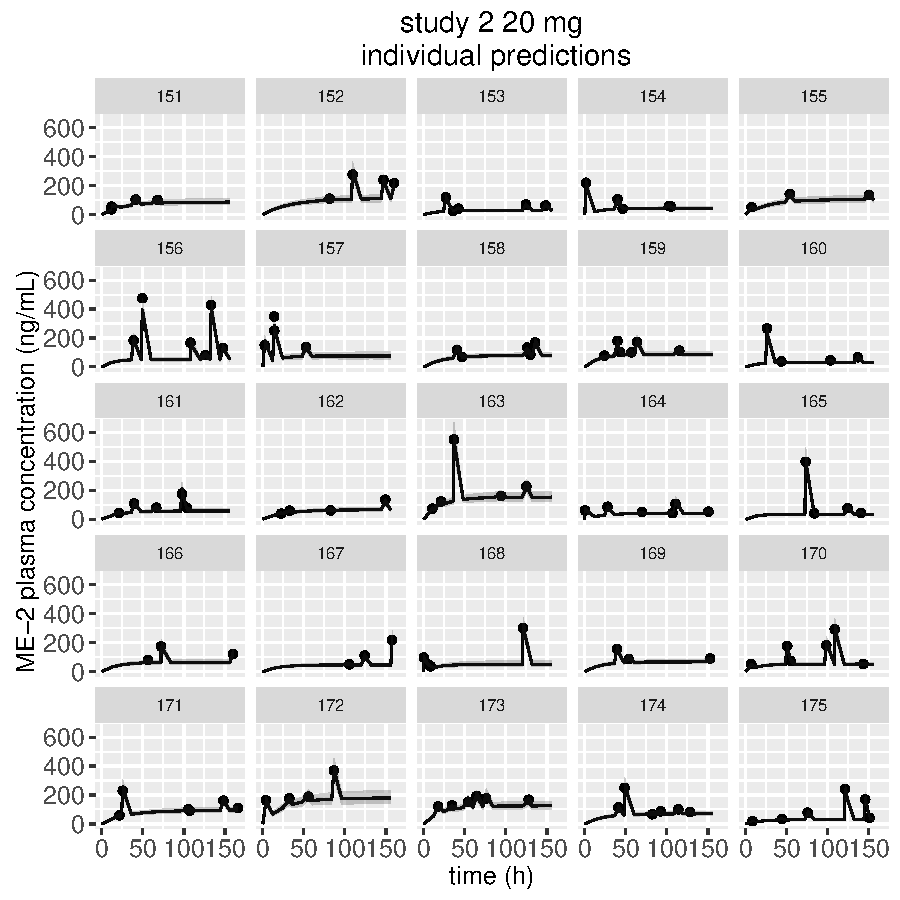
\includegraphics[width=1.5in,trim=0in 0in 0 0in]{graphics/effCptModelTorsten/effCptModelTorstenPlots016.pdf}
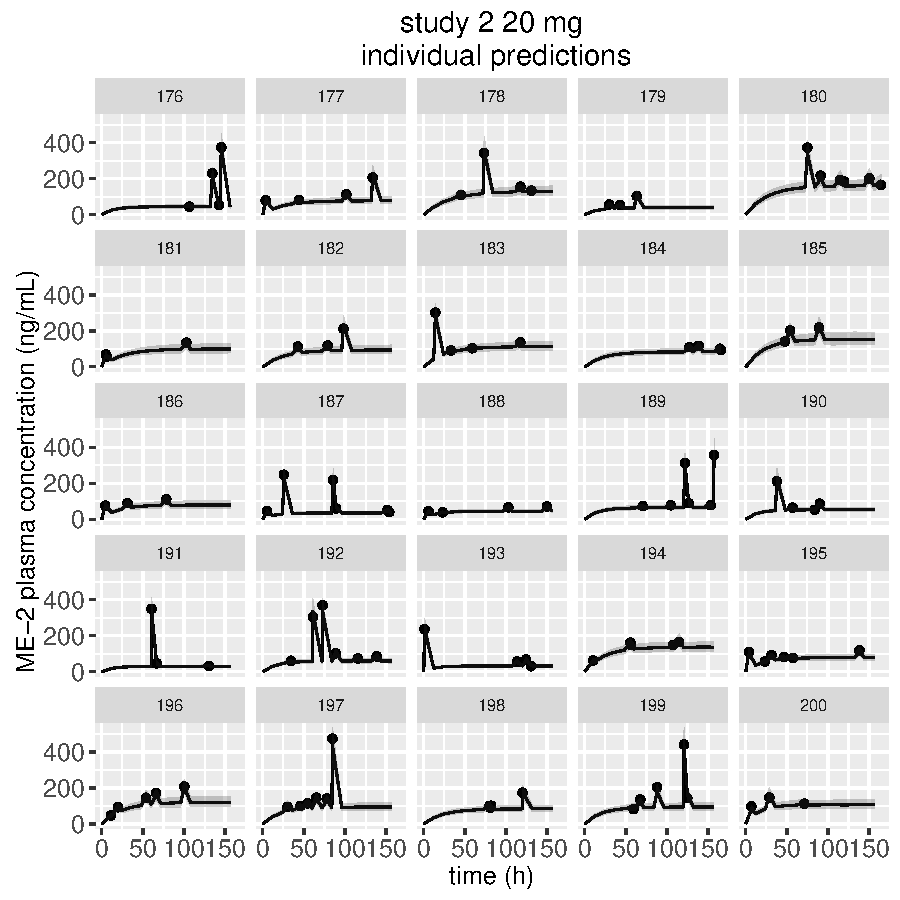
\includegraphics[width=1.5in,trim=0in 0in 0 0in]{graphics/effCptModelTorsten/effCptModelTorstenPlots017.pdf}
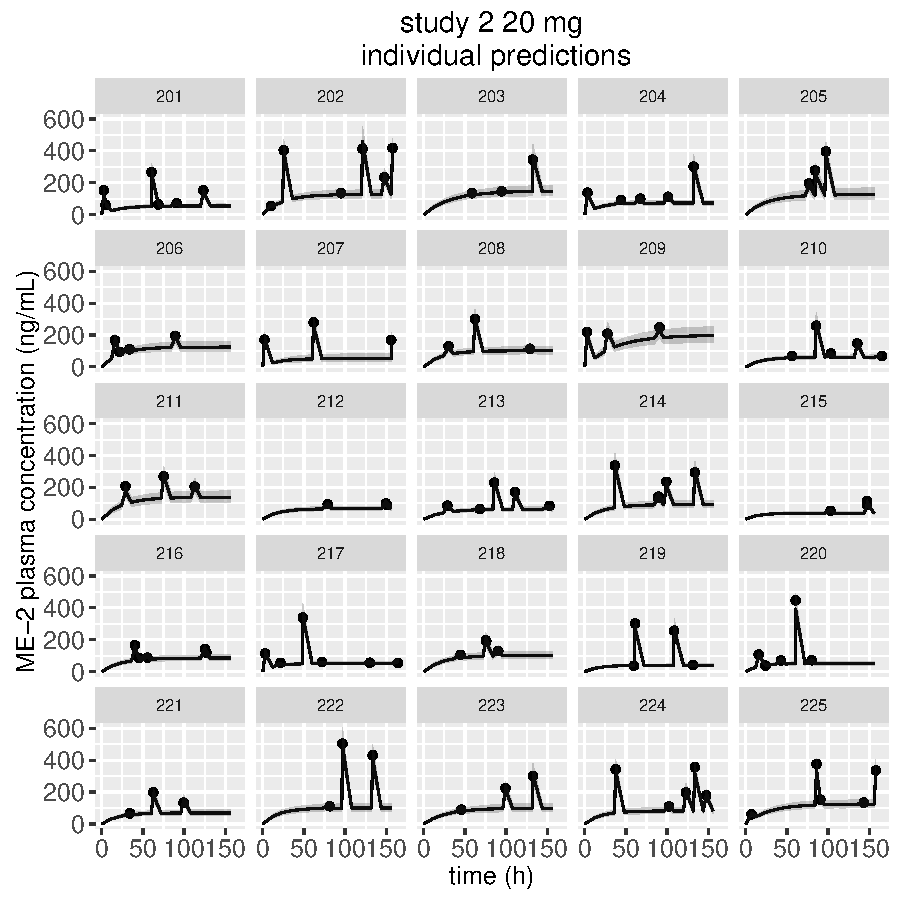
\includegraphics[width=1.5in,trim=0in 0in 0 0in]{graphics/effCptModelTorsten/effCptModelTorstenPlots018.pdf}
\caption{{Predicted (posterior median and 90 \% credible intervals) and observed plasma drug concentrations}}
\label{predictions}
\end{figure}

\begin{figure}[htbp]
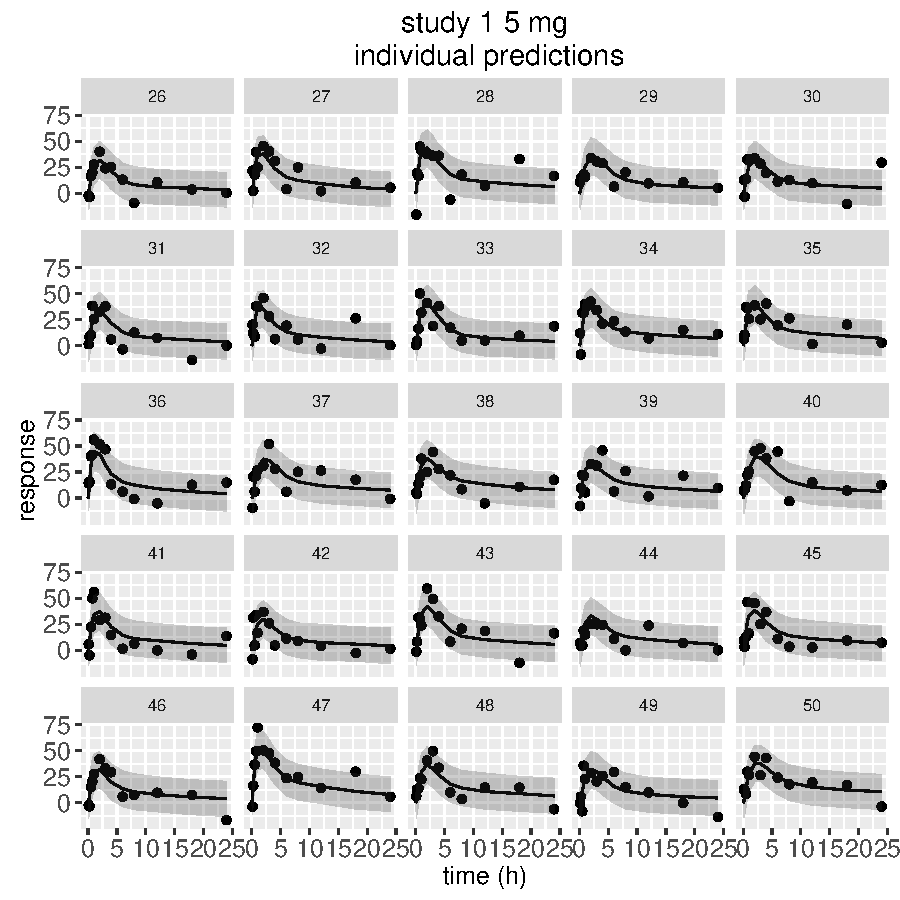
\includegraphics[width=1.5in,trim=0in 0in 0 0in]{graphics/effCptModelTorsten/effCptModelTorstenPlots019.pdf}
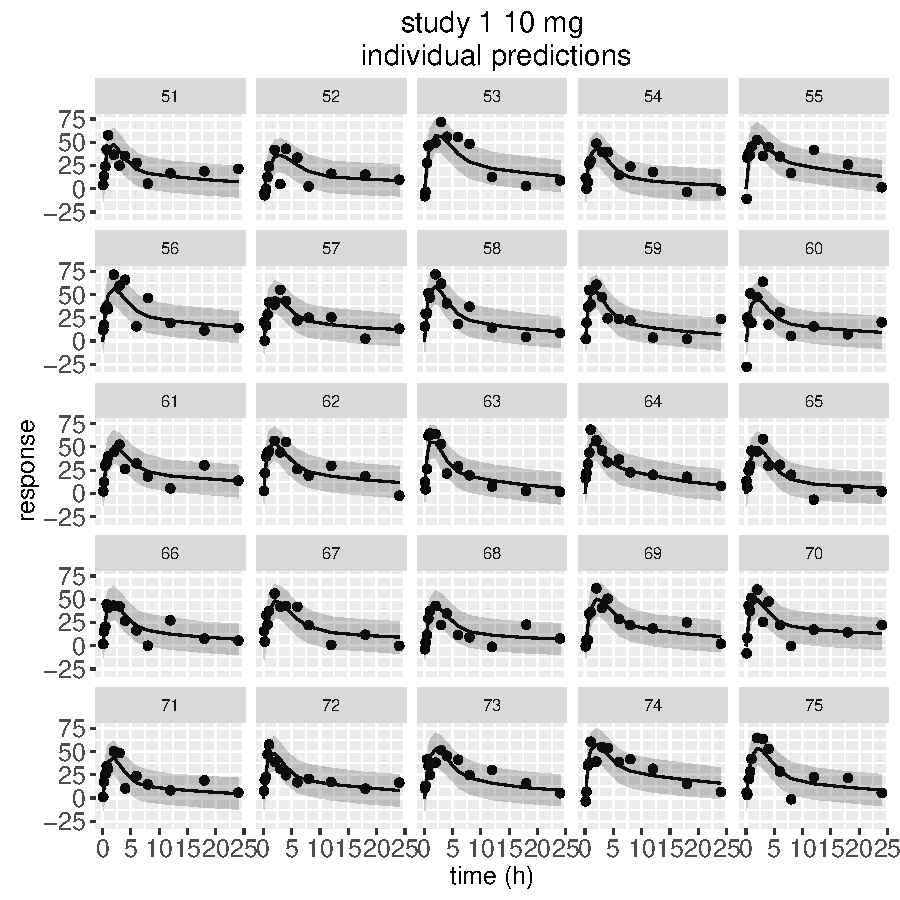
\includegraphics[width=1.5in,trim=0in 0in 0 0in]{graphics/effCptModelTorsten/effCptModelTorstenPlots020.pdf}
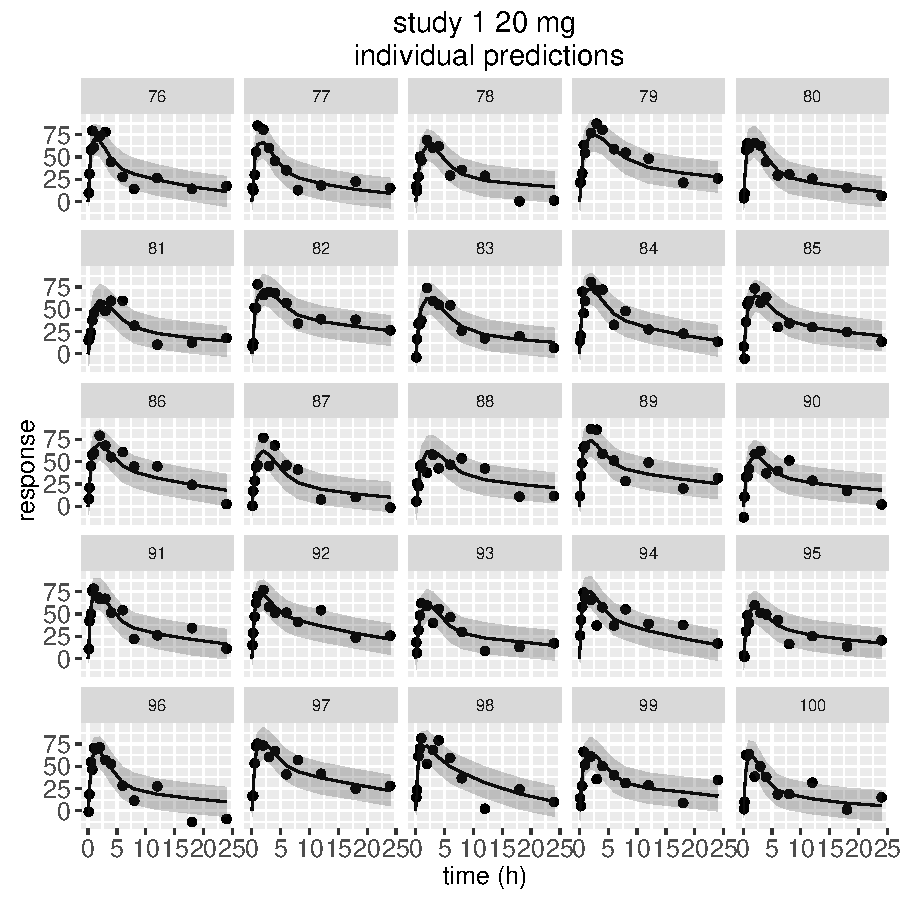
\includegraphics[width=1.5in,trim=0in 0in 0 0in]{graphics/effCptModelTorsten/effCptModelTorstenPlots021.pdf}
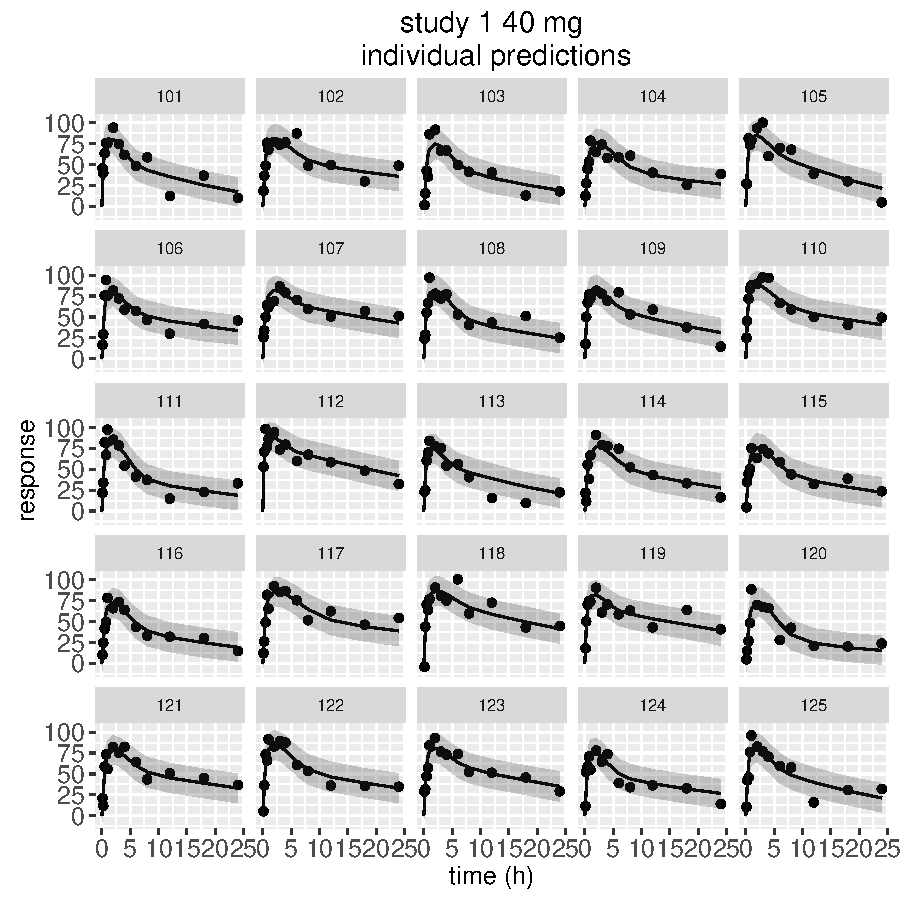
\includegraphics[width=1.5in,trim=0in 0in 0 0in]{graphics/effCptModelTorsten/effCptModelTorstenPlots022.pdf}
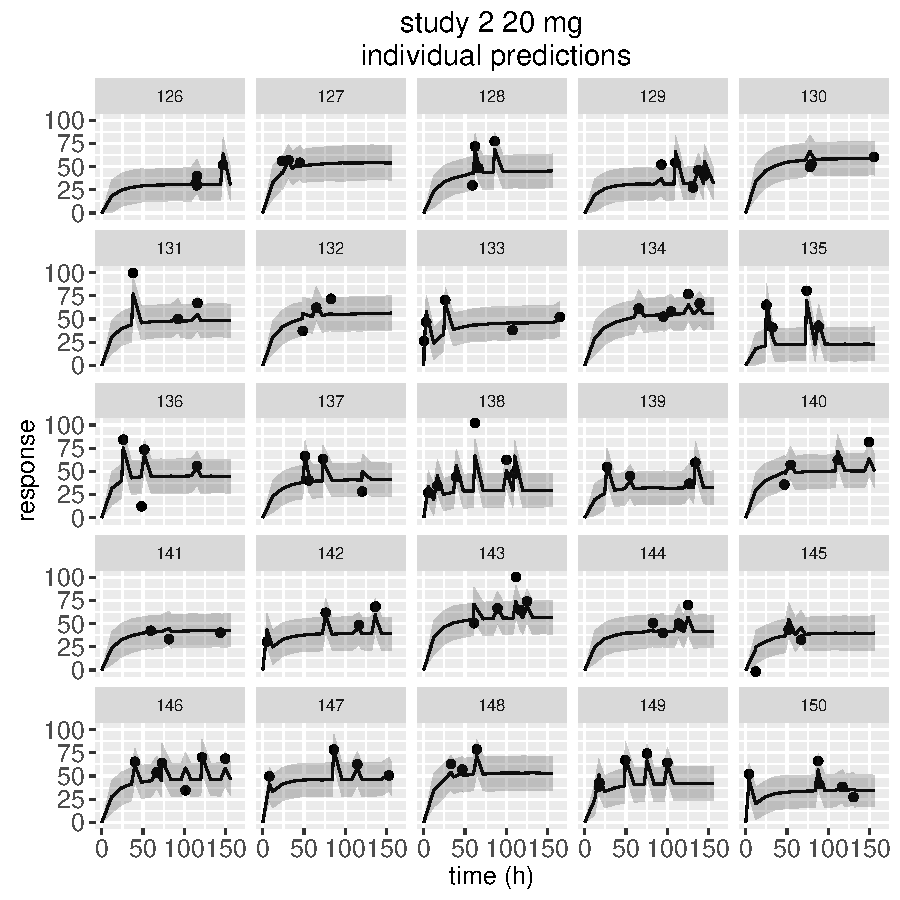
\includegraphics[width=1.5in,trim=0in 0in 0 0in]{graphics/effCptModelTorsten/effCptModelTorstenPlots023.pdf}
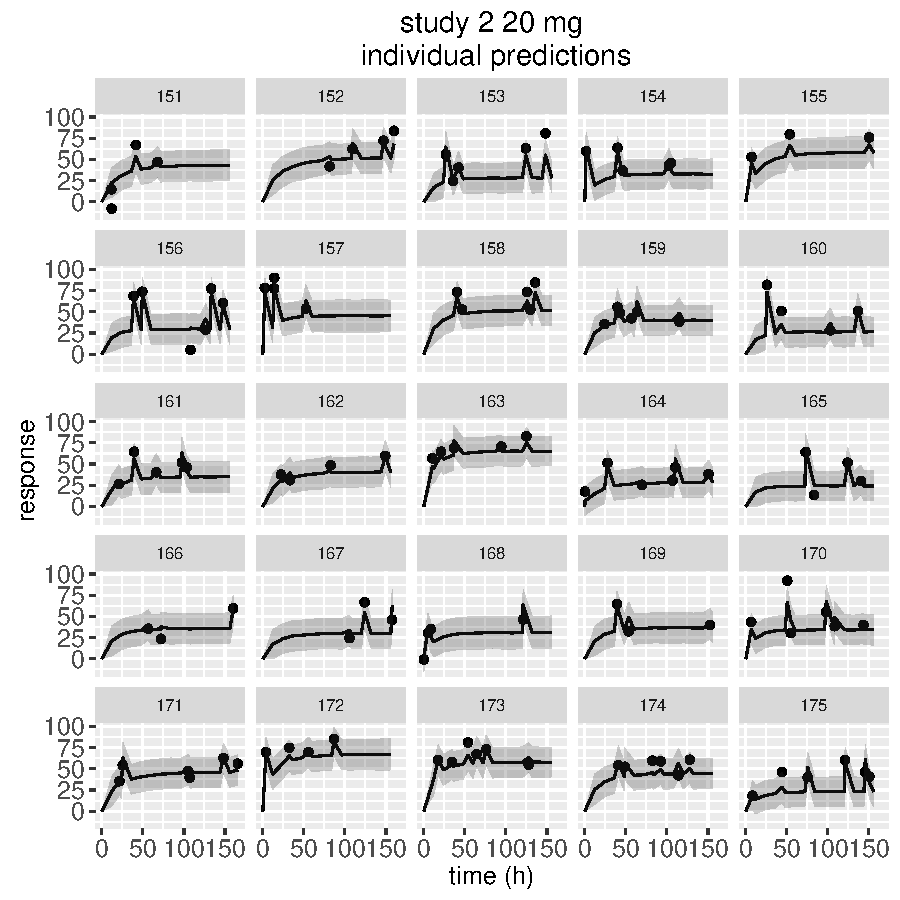
\includegraphics[width=1.5in,trim=0in 0in 0 0in]{graphics/effCptModelTorsten/effCptModelTorstenPlots024.pdf}
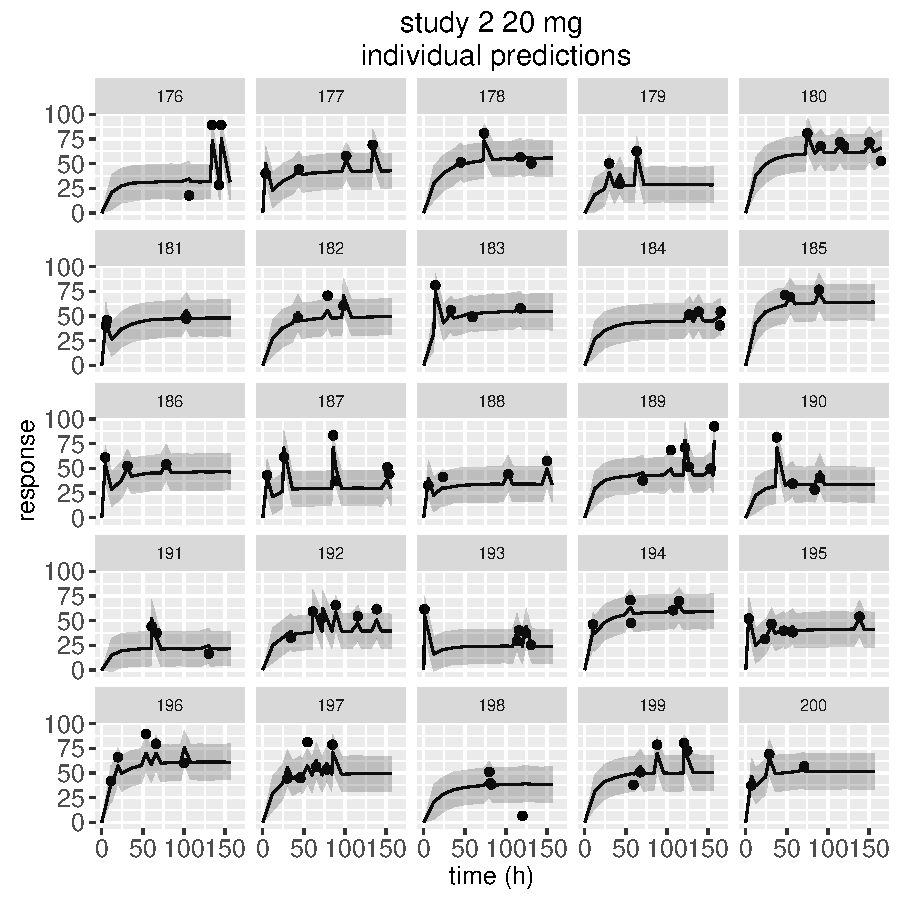
\includegraphics[width=1.5in,trim=0in 0in 0 0in]{graphics/effCptModelTorsten/effCptModelTorstenPlots025.pdf}
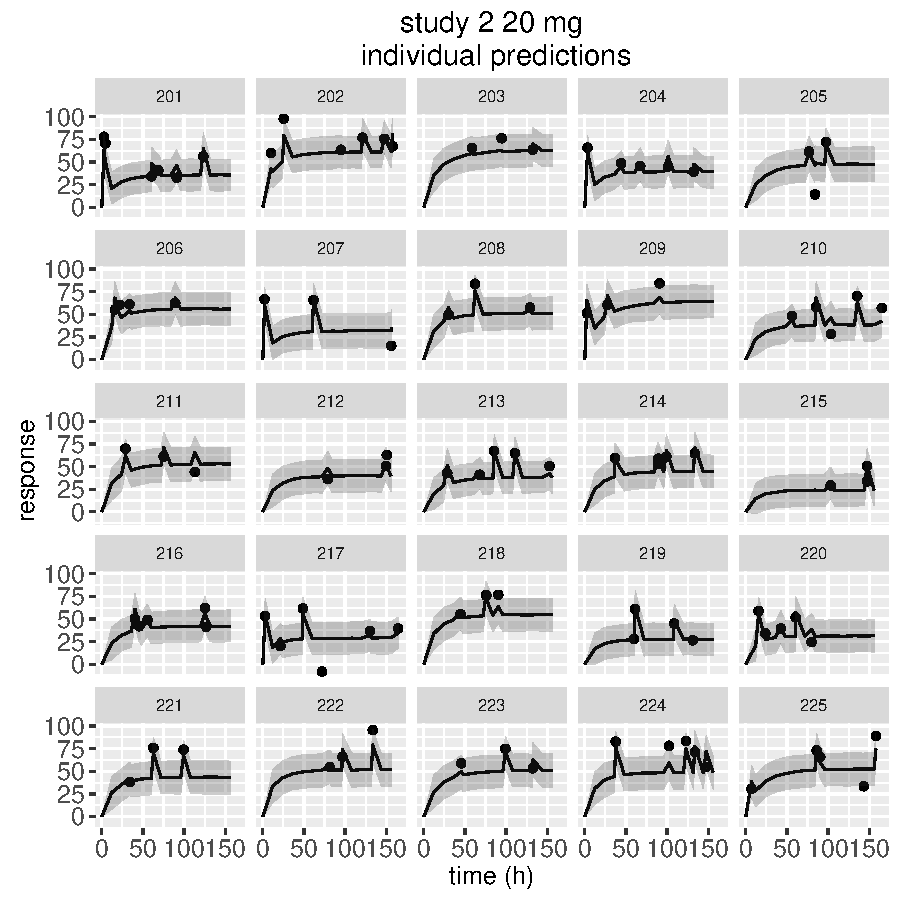
\includegraphics[width=1.5in,trim=0in 0in 0 0in]{graphics/effCptModelTorsten/effCptModelTorstenPlots026.pdf}
\caption{{Predicted (posterior median and 90 \% credible intervals) and observed PD Response}}
\label{predictions}
\end{figure}

\begin{table}[ht]
\centering
\caption{Summary of the MCMC simulations of the marginal posterior distributions of the model parameters}
\begin{tabular}{rrrrrrrrrrr}
  \hline
 & mean & se\_mean & sd & 2.5\% & 25\% & 50\% & 75\% & 97.5\% & n\_eff & Rhat \\ 
  \hline
CLHat & 10.095 & 0.003 & 0.201 & 9.712 & 9.958 & 10.096 & 10.231 & 10.483 & 4000.000 & 0.999 \\
QHat & 14.867 & 0.014 & 0.357 & 14.182 & 14.620 & 14.862 & 15.106 & 15.563 & 678.208 & 1.007 \\
V1Hat & 34.188 & 0.067 & 1.089 & 31.940 & 33.494 & 34.214 & 34.918 & 36.251 & 267.748 & 1.016 \\
V2Hat & 103.562 & 0.076 & 2.925 & 98.031 & 101.600 & 103.455 & 105.472 & 109.583 & 488.296 & 1.001 \\
kaHat & 1.930 & 0.004 & 0.077 & 1.771 & 1.880 & 1.933 & 1.982 & 2.076 & 334.888 & 1.014 \\
ke0Hat & 1.050 & 0.001 & 0.044 & 0.967 & 1.020 & 1.051 & 1.078 & 1.137 & 164.741 & 1.000 \\
EC50Hat & 104.337 & 0.040 & 2.100 & 100.169 & 102.909 & 104.345 & 105.768 & 108.351 & 744.041 & 1.000 \\
sigma & 0.099 & 0.000 & 0.002 & 0.095 & 0.097 & 0.099 & 0.100 & 0.103 & 906.342 & 1.002 \\
sigmaResp & 10.156 & 0.003 & 0.197 & 9.779 & 10.023 & 10.154 & 10.286 & 10.552 & 4000.000 & 1.000 \\
omega[1] & 0.270 & 0.000 & 0.016 & 0.241 & 0.259 & 0.269 & 0.280 & 0.302 & 4000.000 & 1.001 \\
omega[2] & 0.231 & 0.001 & 0.021 & 0.192 & 0.217 & 0.230 & 0.245 & 0.275 & 531.512 & 1.006 \\
omega[3] & 0.219 & 0.002 & 0.031 & 0.158 & 0.199 & 0.218 & 0.238 & 0.281 & 158.198 & 1.017 \\
omega[4] & 0.267 & 0.001 & 0.026 & 0.218 & 0.249 & 0.266 & 0.284 & 0.319 & 684.870 & 1.001 \\
omega[5] & 0.285 & 0.002 & 0.037 & 0.214 & 0.259 & 0.284 & 0.309 & 0.361 & 284.545 & 1.009 \\
omegaKe0 & 0.271 & 0.003 & 0.047 & 0.183 & 0.239 & 0.271 & 0.303 & 0.363 & 217.350 & 1.007 \\
omegaEC50 & 0.213 & 0.001 & 0.021 & 0.174 & 0.199 & 0.213 & 0.227 & 0.255 & 190.193 & 1.000 \\
  \hline
\end{tabular}
\end{table}



\section{Under the Hood Design}
We here discuss some background theory and the design of Torsten at a C++ level.

Our approach is heavily based on the \textit{BUGS model library}, a prototype PKPD model library for WinBUGS (\url{https://bitbucket.org/metrumrg/ bugsmodellibrary/wiki/Home}), developed by Metrum Research Group in 2009.

This section is intended for developers. No knowledge of C++ is required for users.


\subsection*{Computing Amounts in an ODE-based model}
Most PKPD model are based on ODE's that describe how PK and PD amounts evolve over time. For instance, the following ODE's describe drug diffusion in a one compartment model with a first-order absorption from the gut:

\begin{eqnarray*}
\frac{dGUT}{dt} &=& -kaGUT \\ 
\frac{dCENT}{dt} &=& kaGUT - \frac{CL}{V_{1}}CENT
\end{eqnarray*}

If the ODE's fully describe the PKPD system, knowing the state $y_0$ at time $t_0$ fully defines the solution at finite times. Exploiting this property, Torsten calculates how amounts in each compartment evolve from one event to the other. The initial conditions of the ODE system are specified by the previous event, and the ODE's are integrated from $t_{previous} $ to $t_{current}$. 

Note we cannot simply integrate from $t_{first}$ to $t_{last}$ because the ODE's do not describe exterior interventions, such as additional dosing. Torsten treats these interventions independently. Most importantly, Torsten only integrates between $t_0$ and $t_1$ if no exterior interventions occur during this interval. It is key to Properly handle the \textit{event schedule}. 

All five functions in Torsten call the C++ function \texttt{pred}, which does three things:
\begin{enumerate}
  \item Augment the event schedule to include all events that alter the system
  \item Calculate the amounts in each compartment at each event of the augmented schedule
  \begin{itemize}
    \item Compute the \textit{natural} evolution of the system by integrating ODE's
    \item Compute alterations due to exterior interventions
  \end{itemize}
  \item Return the amounts at each event of the original schedule
\end{enumerate}

The Event Schedule depends on the user's input (TIME, EVID, CMT, AMT, RATE, ADDL, II, SS). The event schedule may need to be augmented if, for example, an event specifies a patient receives multiple doses at a regular time interval. Consider: \\

\texttt{TIME = 0, EVID = 1, CMT = 1, AMT = 1500, RATE = 0, ADDL = 4, II = 10, SS = 0} \\

This Event specifies that a time 0 (TIME = 0), a patient receives a 1500 mg (AMT = 1500) drug dose (EVID = 1) in the gut (CMT = 1), and will receive an additional dose every 10 hours (II = 10) until the patient has received a total of 5 doses (ADDL = 4, being the number of additional doses, + 1, the original dose). Such an Event really corresponds to 5 dosing events.

To integrate the ODE's, \texttt{pred} calls \texttt{pred1} (prediction for one event) or \texttt{predSS} (prediction for one event if the system is in a steady state, i.e SS = 1). \texttt{pred1} and \texttt{predSS} are functors and get constructed differently by each Torsten function. Under \texttt{PKModelOneCpt}, \texttt{pred1} analytically computes the solution, while under \texttt{generalCptModel\_rk45} it numerically solves the ODE's.
 
\subsection*{Structure of a Torsten Function} 
Under the structural scheme described above, a Torsten function performs a very simple set of actions:
\begin{enumerate}
  \item Consistent with Stan practices, check the validity of the arguments and of the parameter values
  \item Construct the PKModel object, which contains basic information about the model, such as the number of compartments
  \item Construct the pred1 and predSS functions
  \item Call pred
\end{enumerate}  

Figure 14 shows the C++ code for \texttt{PKModelOneCpt}.

\begin{figure}
\caption{C++ code for the PKModelOneCpt function (abstract)}
\begin{center}
\begin{small}
\begin{fmpage}{\textwidth - .45in}
\begin{lstlisting}[basicstyle=\footnotesize\ttfamily,mathescape=true,flexiblecolumns=true,frame=single,escapeinside=`']

template <typename T0, typename T1, typename T2, typename T3, typename T4> 
Eigen::Matrix <typename promote_args<T0, T1, T2, T3, T4>::type, Eigen::Dynamic,
  Eigen::Dynamic> 
PKModelOneCpt(const std::vector< Eigen::Matrix<T0, Eigen::Dynamic, 1> >& pMatrix, 
			  const std::vector<T1>& time,
			  const std::vector<T2>& amt,
			  const std::vector<T3>& rate,
			  const std::vector<T4>& ii,
			  const std::vector<int>& evid,
			  const std::vector<int>& cmt,
			  const std::vector<int>& addl,
			  const std::vector<int>& ss) {
			  
  using std::vector;
  using Eigen::Dynamic;
  using Eigen::Matrix;
  using boost::math::tools::promote_args;
  using stan::math::check_positive_finite;
  
  PKModel model("OneCptModel"); 
  	 
  // Check arguments
  static const char* function("PKModelOneCpt");
  pmetricsCheck(pMatrix, time, amt, rate, ii, evid, cmt, addl, ss, function, model);
  for(int i=0; i<pMatrix.size(); i++) {
    check_positive_finite(function, "PK parameter CL", pMatrix[i](0,0));
    check_positive_finite(function, "PK parameter V2", pMatrix[i](1,0));
    check_positive_finite(function, "PK parameter ka", pMatrix[i](2,0));
  }
  std::string message4 = ", but must equal the number of parameters in the model: " 
    + boost::lexical_cast<string>(model.GetNParameter()) + "!"; 
  const char* length_error4 = message4.c_str();    
  if (!(pMatrix[0].size() == model.GetNParameter()))
    stan::math::invalid_argument(function,
    "The number of parameters per event (length of a vector in the first argument) is",
    pMatrix[0].size(), "", length_error4);

  // Construct Pred functions for the model.
  Pred1_structure new_Pred1("OneCptModel");
  PredSS_structure new_PredSS("OneCptModel");
  Pred1 = new_Pred1;
  PredSS = new_PredSS; 
  	
  // Construct dummy matrix for last argument of pred
  Eigen::Matrix<double, Dynamic, Dynamic> dummy_system(0,0);

  Matrix <typename promote_args<typename promote_args<T0, T1, T2, T3, T4>::type,
    double>::type, Dynamic, Dynamic> pred;
  pred = Pred(pMatrix, time, amt, rate, ii, evid, cmt, addl, ss, model,
    dummy_ode(), dummy_system);
    
  return pred;
}
\end{lstlisting}
\end{fmpage}
\end{small}
\end{center}
\label{C++ code for the PKModelOneCpt function}
\end{figure}

\subsection*{Implementing Torsten in Stan}
\subsubsection*{Modifications in Stan-math}
All five Torsten functions are located under the \texttt{Torsten} directory, under \texttt{stan/math}. We modified \texttt{rev/math} to include the \texttt{torsten/torsten.hpp} header file. The code can be found on GitHub: \url{https://github.com/charlesm93/math} 

\subsubsection*{Modifications in Stan}
Further modification are done in Stan to expose the Torsten functions to the Stan language. We edited \texttt{function\_signatures.h} to expose \texttt{PKModelOneCpt}, \texttt{PKModelTwoCpt}, and \texttt{linCptModel}. The general compartment model functions are higher-order functions in that they take another function as one of their arguments. They were exposed by directly modifying the grammar files, following very closely the example of \texttt{integrate\_ode\_rk45} and \texttt{integrate\_ode\_bdf}.

The code can be found on GitHub:  \url{https://github.com/charlesm93/stan}

%\subsection{Acknowledgments and Thanks}

\end{document}
